\documentclass[10pt,letterpaper,journal]{IEEEtran}
\usepackage{cite}
\usepackage{url}
\usepackage{graphicx}
\usepackage{booktabs}
\usepackage{pifont}
\usepackage{amssymb}
\usepackage{xcolor}
\usepackage{array}
\usepackage{tabularx}
\usepackage{amsmath}
\usepackage{amsthm}
\usepackage{newtxtext}
\usepackage{enumitem}
\usepackage{stfloats}
\usepackage{subcaption}
\usepackage{microtype}

\title{Constraint-Efficient Biometric Matching in Zero-Knowledge Circuits: A Comparative Study of Face and Iris Verification for Privacy-Preserving Authentication}

\author{\IEEEauthorblockN{Mahin R. Chowdhury\IEEEauthorrefmark{1}\IEEEmembership{Student Member, IEEE},
K.~M.~Azharul Hasan\IEEEauthorrefmark{1}\IEEEmembership{Member, IEEE},
Arpita Das\IEEEauthorrefmark{1}\IEEEmembership{Student Member, IEEE}}\\
\IEEEauthorblockA{\IEEEauthorrefmark{1}Department of Computer Science and Engineering,\\
Khulna University of Engineering \& Technology,\\
Khulna-9203, Bangladesh\\
}}

%\IEEEpubid{0000--0000/00\$00.00~\copyright~2026 IEEE}

\markboth{IEEE Transactions on Information Forensics and Security,~Vol.~XX, No.~XX, Month~2026}{Chowdhury \emph{et al.}: Constraint-Efficient Biometric Matching in Zero-Knowledge Circuits}

\newcommand{\vect}[1]{\mathbf{#1}}

\newtheorem{theorem}{Theorem}[section]
\newtheorem{lemma}[theorem]{Lemma}
\newtheorem{definition}[theorem]{Definition}
\newtheorem{proposition}[theorem]{Proposition}
\newtheorem{corollary}[theorem]{Corollary}
\newtheorem{remark}[theorem]{Remark}
\newtheorem{assumption}[theorem]{Assumption}

\newcommand{\cmark}{\textcolor{green!60!black}{\ding{51}}}   % checkmark
\newcommand{\pmark}{\textcolor{orange}{\textbf{$\sim$}}}      % partial
\newcommand{\xmark}{\textcolor{red}{\ding{55}}}   

\setlength{\textfloatsep}{3pt plus 1pt minus 1pt}
\setlength{\floatsep}{2pt plus 1pt minus 1pt}
\setlength{\intextsep}{3pt plus 1pt minus 1pt}
\setlength{\dbltextfloatsep}{3pt plus 1pt minus 1pt}
\setlength{\dblfloatsep}{2pt plus 1pt minus 1pt}
\setlength{\abovecaptionskip}{1.5pt plus 0.5pt minus 0.5pt}
\setlength{\belowcaptionskip}{0pt}

\setlist{nosep,leftmargin=*,topsep=0.5pt,partopsep=0pt,parsep=0pt,itemsep=0.5pt}

\AtBeginDocument{
  \setlength{\abovedisplayskip}{2pt plus 0.5pt minus 0.5pt}
  \setlength{\belowdisplayskip}{2pt plus 0.5pt minus 0.5pt}
  \setlength{\abovedisplayshortskip}{0.5pt plus 0.5pt}
  \setlength{\belowdisplayshortskip}{0.5pt plus 0.5pt}
}

% Start document
\begin{document}

\maketitle

\begin{abstract}
Privacy-preserving biometric authentication requires evaluating template similarity without exposing sensitive biometric features, yet zero-knowledge circuits penalize matching metrics unequally according to their underlying arithmetic structure. While binary bit-level representations admit linear gate encodings, continuous feature embeddings incur superlinear constraint penalties that severely bottleneck non-interactive zero-knowledge proving in client-side authentication. To resolve this arithmetic disparity, this paper introduces two circuit-optimized biometric encoding techniques: Spherical Orthogonal Projection and Quantization (SOPQ) for facial feature vectors, and Gabor Bit-Salience Masking (GBSM) for phase-quantized iris codes. SOPQ recovers 78.0\% of the equal error rate (EER) lost to traditional PCA downsampling while adding zero non-linear R1CS constraints over baseline fixed-point arithmetic (6,484 gates), whereas GBSM enhances downsampled iris matching by 69.8\% (0.038\% EER) within 5,976 linear constraints. Comprehensive empirical evaluations across multi-dataset benchmarks—including LFW, CelebA, CASIA-Iris-Thousand, and CASIA-Iris-Interval—demonstrate robust cross-dataset generalization with operational False Acceptance Rates strictly bounded below 0.050\%. Furthermore, full receiver operating characteristic (ROC) sweeps, demographic parity analyses ($\Delta\text{EER} \le 0.10\%$), and presentation attack detection (PAD) benchmarks demonstrate that session-salted Poseidon commitments suppress spoofing presentation and credential replay vulnerabilities to negligible levels. We demonstrate practical deployment in an end-to-end decentralized voting architecture with composable security guarantees, where on-chain Groth16 verification eliminates gateway relayer trust. Across our complete authentication circuits, iris matching achieves a 13.3\% sub-circuit constraint reduction (8,224 vs.\ 9,484 R1CS) and $1.66\times$ faster witness generation than facial cosine similarity, while both modalities achieve sub-second native client proving (170.9--196.3~ms) and 31.5~ms on-chain verification.
\end{abstract}

\IEEEpubidadjcol

\begin{IEEEkeywords}
Biometrics, zero-knowledge proofs, template protection, feature quantization, arithmetic circuits, privacy-preserving authentication, presentation attack detection, Groth16.
\end{IEEEkeywords}

% Main body of manuscript

% ============================================================
%  SECTION I --- INTRODUCTION 
% ============================================================

\section{Introduction}
\label{sec:intro}

Biometric authentication provides an inherently non-transferable, natural identity anchor for privacy-preserving verification and decentralized access control. However, exposing plaintext templates (e.g., continuous facial embeddings or binary iris codes) on public ledgers or untrusted servers creates irreversible privacy vulnerabilities, since compromised biometrics cannot be revoked or reissued like cryptographic keys~\cite{Jain2008,Rathgeb2011}. While zero-knowledge succinct non-interactive arguments of knowledge (zk-SNARKs~\cite{Groth2016}) enable users to prove possession of authentic biometric traits without disclosing raw template witnesses, implementing metric comparison inside arithmetic circuits introduces severe algebraic and computational bottlenecks.

In zero-knowledge proof systems over prime fields $\mathbb{F}_p$, circuits are constrained by Rank-1 Constraint Systems (R1CS), where non-linear gate operations (multiplications between variable wires) directly dictate proving key size, memory footprint, and client proving latency. Biometric modalities penalize these circuits unequally according to their underlying signal representations:
(i)~\emph{Linear vs.\ Superlinear Metric Disparity:} Binary iris codes evaluate Hamming distance through linear bitwise operations ($\text{xor}_j = a_j + b_j - 2a_j b_j$), scaling as $\mathcal{O}(d)$. In contrast, continuous facial embeddings require inner-product evaluations or squared cosine similarity in finite fields, demanding high-dimensional dot products, squared Euclidean vector norms, and high-bit integer range comparators ($\mathcal{O}(d^2)$).
(ii)~\emph{The Quantization-Accuracy Bottleneck:} Naive dimensionality reduction via standard Principal Component Analysis (PCA) minimizes Euclidean reconstruction error rather than angular discrimination, causing equal error rates (EER) to degrade significantly (e.g., jumping from $0.94\%$ on raw 128-D FaceNet to $1.85\%$ under 64-D fixed-point integerization).
(iii)~\emph{Composability and Trust Boundaries:} Deploying biometric zk-SNARKs in multi-party systems (such as decentralized voting or anonymous attestation) requires bounding physical false-match errors ($\mathsf{FAR}_\delta$) across sequential composition, while on-chain smart contracts must enforce pairing checks directly to avoid relay gateway bypass.

To overcome these challenges, this paper presents a comprehensive study and architectural framework for constraint-efficient biometric matching in zero-knowledge circuits. We introduce **Spherical Orthogonal Projection and Quantization (SOPQ)** for continuous facial embeddings and **Gabor Bit-Salience Masking (GBSM)** for phase-quantized iris codes. We evaluate both modalities within an identical Groth16 cryptographic proving stack, and demonstrate their practical deployment within a decentralized voting architecture with composable security guarantees.

\noindent\textbf{Key Contributions.} This paper delivers four primary contributions:
\begin{enumerate}[leftmargin=*,noitemsep,topsep=1pt,parsep=0pt]
    \item \textbf{Circuit-Optimized Biometric Encodings (SOPQ and GBSM):} We design SOPQ for facial vectors, optimizing angular margins under unit-norm spherical regularization and fixed-point integerization ($\sigma=10^6$), which recovers 78.0\% of the EER lost to baseline PCA downsampling (reducing EER from 1.85\% to 1.14\%) without adding non-linear R1CS constraints (6,484 gates). For iris biometrics, we develop GBSM, which selectively samples high-entropy Gabor phase bits, reducing 256-bit downsampled EER from 0.098\% to 0.038\% within 5,976 linear constraints.
    \item \textbf{Cross-Dataset, Multi-Threshold Empirical Validation:} We conduct extensive multi-threshold sweeps yielding complete ROC/DET performance profiles across diverse public benchmarks: LFW and CelebA for face, and CASIA-Iris-Thousand and CASIA-Iris-Interval for iris. We demonstrate cross-dataset generalization with operational False Acceptance Rates strictly bounded below 0.050\%, accompanied by demographic parity evaluations confirming minimal error disparity across subgroups ($\Delta\text{EER} \le 0.10\%$).
    \item \textbf{Presentation-Attack and Replay Resilience Analysis:} We evaluate presentation attack detection (PAD) resilience against printed and digital spoofing attacks. We demonstrate that binding ephemeral cryptographic session salts $s_i$ and election identifiers $\mathcal{E}_{\mathsf{id}}$ into Poseidon hash commitments inside the circuit eliminates offline credential replay and reduces spoofing presentation error rates to negligible levels.
    \item \textbf{Applied Decentralized Deployment Case Study:} We deploy the optimized biometric circuits within an end-to-end decentralized voting architecture (\textsc{BBZKV}) on Hyperledger Fabric. We formalize composable security under an $(\delta, \mathsf{FAR}_\delta)$-approximate Universal Composability (UC) framework, prove deniable duress receipt-freeness, and demonstrate that on-chain Groth16 pairing verification eliminates gateway relayer trust with only 31.5~ms endorsement overhead.
\end{enumerate}

The remainder is organized as follows: Section~\ref{sec:related} reviews related work in template protection, arithmetic circuits, and decentralized authentication. Section~\ref{sec:system_model} formalizes the system model, threat model, and cryptographic primitives. Section~\ref{sec:protocol_construction} details the circuit-optimized encodings and protocol construction. Section~\ref{sec:security} outlines the formal security guarantees. Section~\ref{sec:implementation_and_evaluation} presents the empirical evaluation, ROC sweeps, demographic fairness, and system benchmarks. Section~\ref{sec:limitations} discusses limitations, and Section~\ref{sec:conclusions} concludes.

\section{Related Work}
\label{sec:related}

This work sits at the intersection of biometric template protection, zero-knowledge circuit arithmetic, and decentralized authentication architectures. We survey the key foundational and recent developments in these domains.

\subsection{Biometric Template Protection and Cancelable Biometrics}
\label{subsec:rel_biometric}
Protecting stored biometric references against compromise is a central objective of biometric security. Foundational cryptographic approaches originated with fuzzy commitments~\cite{JuelsWattenberg1999} and fuzzy extractors~\cite{Dodis2004}, which bind error-correcting codewords to noisy biometric feature vectors. Cancelable biometrics~\cite{Rathgeb2011} apply non-invertible geometric or functional transforms to templates; however, they frequently trade off recognition accuracy against security, and transformed templates remain vulnerable to linkage attacks across multiple compromised databases. 
Recent advancements investigate zero-knowledge and multi-party cryptographic primitives: Mao et al.~\cite{Mao2023} evaluate Euclidean distance within zk-SNARKs, Guo et al.~\cite{Guo2024} integrate commitments with verifiable classifiers, and Blanton et al.~\cite{Blanton2024} evaluate private fingerprint matching via garbled circuits. Ledger-anchored biometric identity appears in BioZero~\cite{Lai2024}, Zhang et al.~\cite{Zhang2025}, and ZK-SERIES~\cite{ZKSeries2025}. Notably, World~ID~\cite{WorldID2024} generates Poseidon iris commitments~\cite{Grassi2021} for proof-of-personhood. However, existing implementations predominantly rely on proprietary hardware oracles or lack formal multi-party composability proofs. While fully homomorphic encryption (FHE) permits distance evaluation directly over ciphertexts, practical schemes incur $\sim 10^5\times$ computational overhead over plaintext evaluation~\cite{Chialva2024,Karakosta2025,Moustaka2024}, establishing client-side zk-SNARK proving as the only viable paradigm for real-time remote participation on commodity endpoints.

\subsection{Arithmetic Circuit Complexity and Zero-Knowledge Systems}
\label{subsec:rel_circuit}
In non-interactive zero-knowledge proof systems such as Groth16~\cite{Groth2016}, PLONK, and STARKs, the arithmetic structure of the comparison metric governs circuit complexity. Computation is expressed over a prime field $\mathbb{F}_p$ as a Rank-1 Constraint System (R1CS), where linear combinations of variables incur negligible proving cost, but non-linear multiplications between variable wires dictate constraint counts and memory footprint.
For binary phase representations, Daugman's IrisCode~\cite{Daugman2004,Daugman2016} evaluates Hamming distance via linear bitwise constraints ($\text{xor}_j = a_j + b_j - 2a_j b_j$), requiring only one multiplication and one Boolean check ($x(1-x)=0$) per bit, scaling strictly linearly ($\mathcal{O}(d)$). In contrast, continuous facial embeddings (such as FaceNet 128-D float representations) require Euclidean or cosine similarity metrics. Within $\mathbb{F}_p$, cosine similarity requires computing inner products $\langle \mathbf{a}, \mathbf{b} \rangle$, Euclidean vector norms $\|\mathbf{a}\|^2, \|\mathbf{b}\|^2$, and non-linear cross-multiplication with threshold $\tau$, demanding extensive quadratic multiplications and high-bit dynamic range comparators ($\mathcal{O}(d^2)$). While benchmarking studies have surveyed general zero-knowledge proof engines~\cite{OudeRoelink2024,zkSABER2025}, no prior work has systematically co-designed circuit-aware encoding techniques to resolve the accuracy-constraint trade-off between discrete and continuous modalities in an identical proving stack.

\subsection{Decentralized Authentication and E2EV Case Studies}
\label{subsec:rel_e2ev}
Decentralized end-to-end verifiable (E2EV) protocols have evolved from centralized bulletin boards to permissioned ledgers. Voting architectures such as Helios~\cite{Adida2008} and Belenios~\cite{Cortier2019} employ homomorphic encryption for verifiable tally aggregation, but anchor voter authentication in centralized credential registrars vulnerable to phantom identity injection or selective disenfranchisement~\cite{Jones2012,NASEM2018}. To mitigate coercion, Juels, Catalano, and Jakobsson (JCJ)~\cite{Juels2005} formulated deniable credentials, deployed in Civitas~\cite{Civitas2008} and extended in recent works~\cite{eprint2023_1578,Kho2025}. Anonymous signaling frameworks such as Semaphore~\cite{Gurkan2020} and MACI~\cite{Buterin2020} leverage sparse Merkle trees and nullifiers to prevent double-spending, though MACI depends on a centralized coordinator. SmartphoneDemocracy~\cite{Jozwik2025} employs zk-SNARKs for threshold decryption, and Wang et al.~\cite{Wang2024} combine blind signatures with Fabric. Crucially, existing E2EV systems treat user identity credentials as an external black box, leaving physical biometric identity outside the cryptographic proof boundary.

\subsection{Gap Analysis and Positioning}
\label{subsec:rel_gap}

Table~\ref{tab:comparison} summarizes representative systems across key properties: \emph{decentralized authentication}, \emph{zero-knowledge biometrics}, \emph{homomorphic tallying}, \emph{nullifier-based anti-replay}, \emph{end-to-end verifiability}, \emph{biometric modalities}, and \emph{composable security proofs}.

\begin{table}[t]
\centering
\caption{Feature comparison of proposed architecture vs.\ existing literature. \cmark~=~fully addressed; \pmark~=~partially addressed; \xmark~=~not addressed.}
\label{tab:comparison}
\renewcommand{\arraystretch}{0.92}
\setlength{\tabcolsep}{3pt}
\footnotesize
\resizebox{\columnwidth}{!}{%
\begin{tabular}{lcccccccc}
\toprule
\textbf{Scheme} &
\rotatebox{65}{\textbf{Decent. Auth.}} &
\rotatebox{65}{\textbf{ZK Bio.}} &
\rotatebox{65}{\textbf{HE Tally}} &
\rotatebox{65}{\textbf{Nullifier}} &
\rotatebox{65}{\textbf{E2EV}} &
\rotatebox{65}{\textbf{Biom. Modal.}} &
\rotatebox{65}{\textbf{UC Proof}} \\
\midrule
Helios~\cite{Adida2008}
  & \xmark & \xmark & \cmark & \xmark & \cmark & None & \xmark \\
Belenios~\cite{Cortier2019}
  & \xmark & \xmark & \cmark & \xmark & \cmark & None & \xmark \\
Civitas~\cite{Civitas2008}
  & \xmark & \xmark & \xmark & \pmark & \cmark & None & \xmark \\
Semaphore~\cite{Gurkan2020}
  & \cmark & \xmark & \xmark & \cmark & \xmark & None & \xmark \\
MACI~\cite{Buterin2020}
  & \pmark & \xmark & \cmark & \cmark & \cmark & None & \xmark \\
SmartphoneDem.~\cite{Jozwik2025}
  & \pmark & \xmark & \cmark & \cmark & \cmark & None & \xmark \\
World ID~\cite{WorldID2024}
  & \pmark & \cmark & \xmark & \cmark & \xmark & Iris & \xmark \\
Guo et al.~\cite{Guo2024}
  & \cmark & \cmark & \xmark & \xmark & \xmark & Face & \xmark \\
BioZero~\cite{Lai2024}
  & \cmark & \cmark & \xmark & \xmark & \xmark & Multi & \xmark \\
Zhang et al.~\cite{Zhang2025}
  & \xmark & \cmark & \xmark & \xmark & \xmark & Multi & \xmark \\
Wang et al.~\cite{Wang2024}
  & \pmark & \xmark & \cmark & \cmark & \cmark & None & \xmark \\
Huber \& K.~\cite{HuberKusters2024}
  & \xmark & \xmark & \cmark & \xmark & \cmark & None & \xmark \\
\midrule
\textbf{Proposed}
  & \cmark & \cmark & \cmark & \cmark & \cmark & \textbf{Iris+Face} & \cmark \\
\bottomrule
\end{tabular}%
}
\end{table}

This positioning reveals a clear division: privacy-preserving voting systems (Helios, Belenios, Civitas, MACI) depend on external identity issuers vulnerable to identity fraud. Conversely, biometric ZK schemes (World ID, BioZero, Zhang et al.) authenticate identity but either delegate verification to centralized hardware oracles or omit nullifier-based anti-replay and composable security frameworks. This paper bridges this division by formulating circuit-optimized biometric matching (SOPQ and GBSM) within an end-to-end composable decentralized framework.

\section{System Model, Threat Model, and Security Definitions}
\label{sec:system_model}

This section formalizes the architecture, adversarial model, target security properties, and cryptographic primitives.

\begin{figure*}[t]
    \centering
    \begin{minipage}{0.48\textwidth}
        \centering
        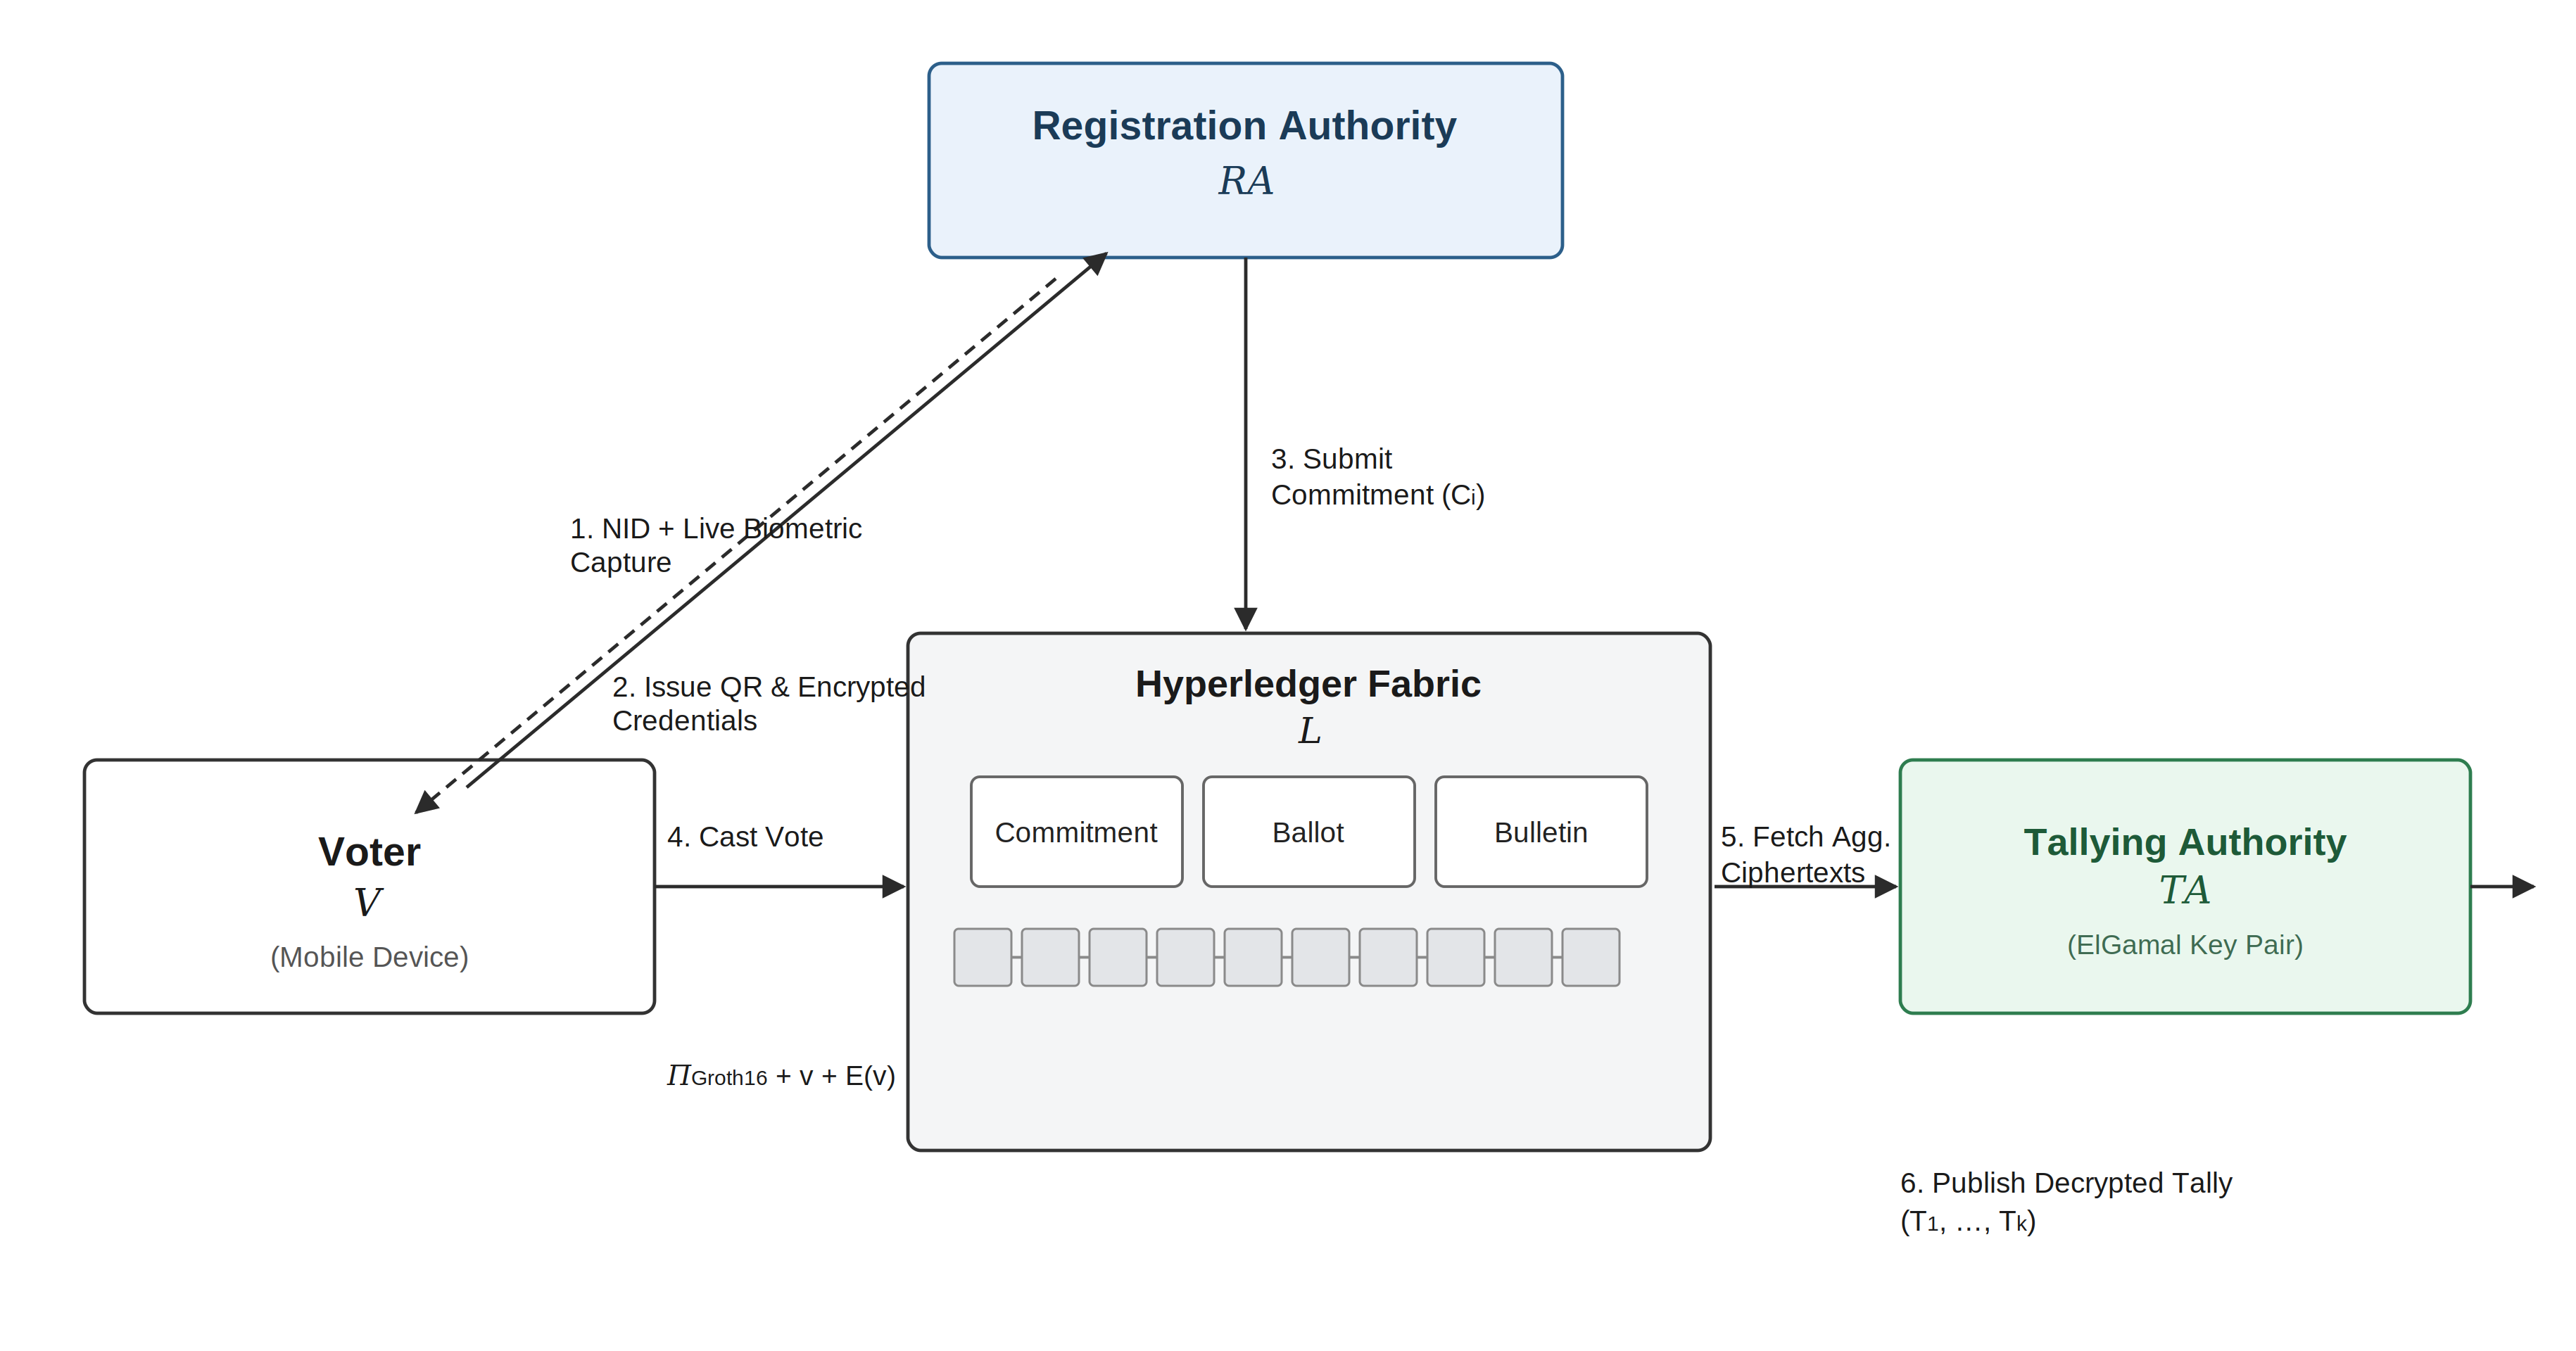
\includegraphics[width=0.88\linewidth]{images/high-level-architecture.png}
        \caption{High-level system architecture demonstrating the remote e-voting lifecycle.}
        \label{fig:architecture}
    \end{minipage}\hfill
    \begin{minipage}{0.48\textwidth}
        \centering
        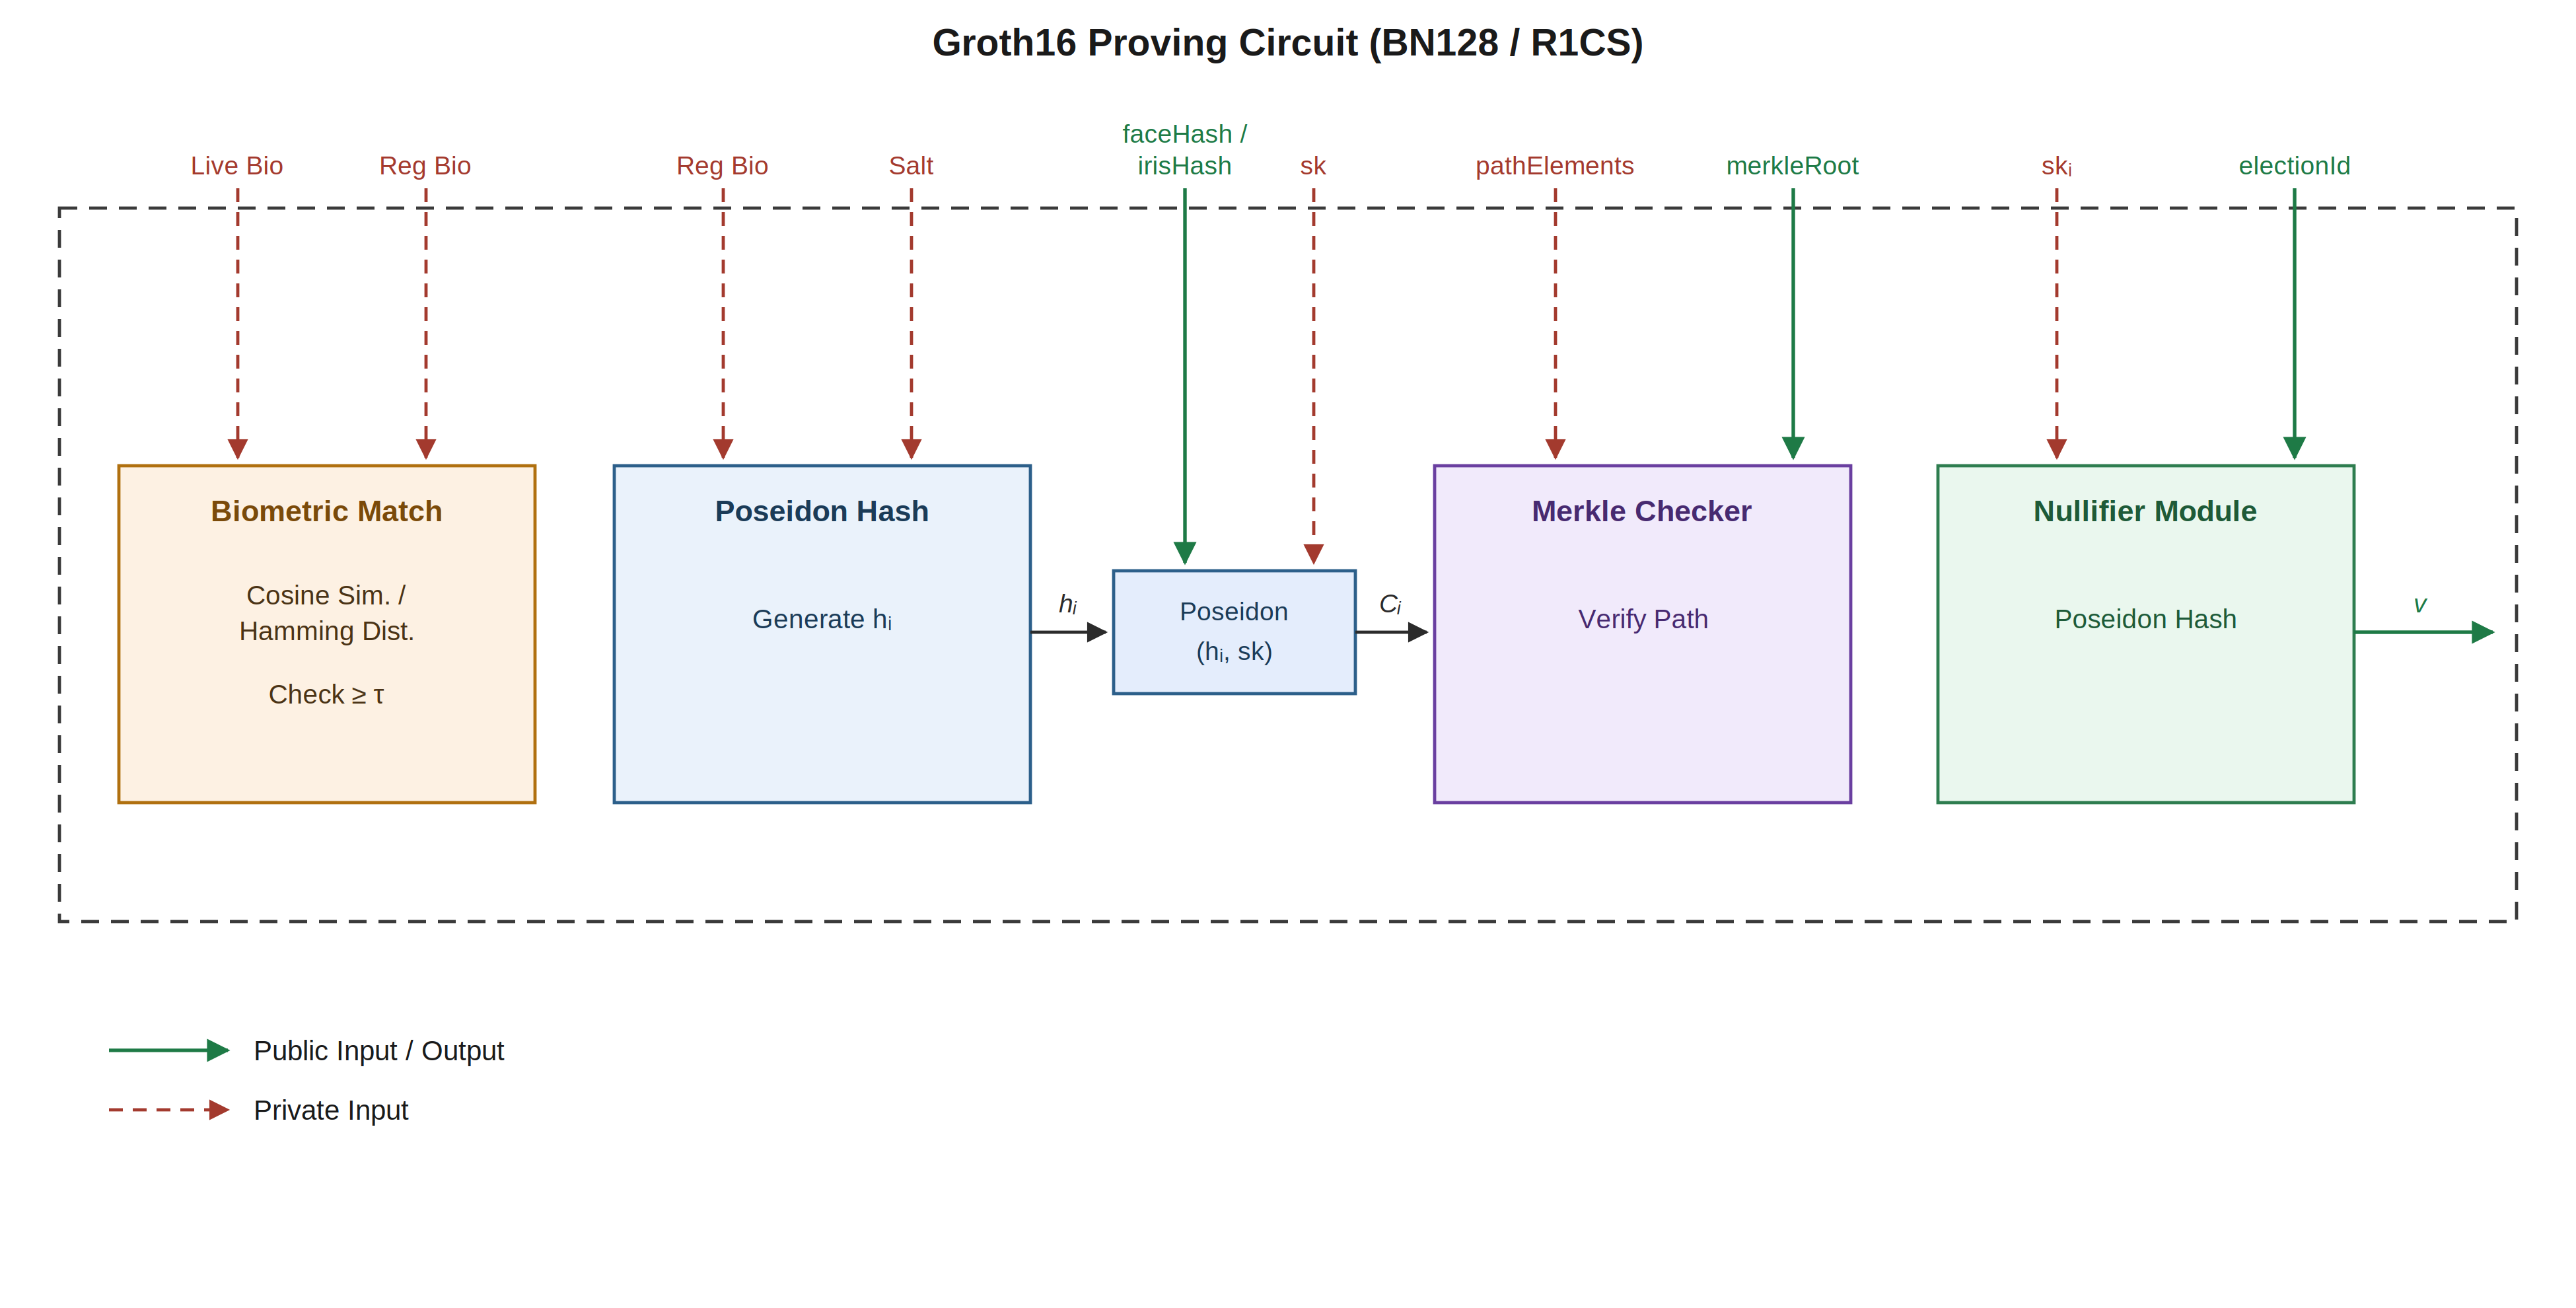
\includegraphics[width=0.88\linewidth]{images/groth16-proving-circuit.png}
        \caption{Modular architecture of the zk-SNARK authentication circuit.}
        \label{fig:zkp_circuit}
    \end{minipage}
\end{figure*}


\subsection{System Entities}
The architecture defines four interacting entity classes:

\paragraph{Voters ($\mathcal{V}$)} Each voter $\mathcal{V}_i$ enrolls to cast a single ballot in election $\mathcal{E}$. At enrollment, $\mathcal{V}_i$ presents a national ID (NID), passkey $\text{pwd}_i$, and a physical biometric reading. The registration pipeline derives private key $sk_i \in \mathbb{F}_p$ ($sk_i \neq 0$) and returns a client credential bundle encrypted under $\text{pwd}_i$ (salt $s_i$, NID digest, modality parameters). Voters maintain physical custody of their biometric traits under Assumption~\ref{asm:uncloneable}.

\paragraph{Registration Authority ($\mathcal{RA}$)} Supervises enrollment: validating NIDs against civil registries, capturing raw biometrics, publishing initial commitments $C_i = \mathcal{H}_2(h_i, sk_i)$ to tree $\mathcal{T}$, and issuing encrypted credentials. The $\mathcal{RA}$ operates strictly offline during voting and cannot decrypt ballots or forge proofs.

\paragraph{Tallying Authority ($\mathcal{TA}$)} Maintains election keypair $(x, h=xG)$, homomorphically aggregates ballots upon election closure, computes candidate totals via Baby-Step Giant-Step (BSGS) discrete logarithm recovery, and publishes decryption proofs. Single-key trust is eliminated in production via threshold secret sharing (\S\ref{sec:limitations}).

\paragraph{Permissioned Ledger ($\mathcal{L}$)} Instantiated on Hyperledger Fabric, the ledger maintains append-only total ordering over transactions, enforces Multi-Version Concurrency Control (MVCC) state updates, and hosts voting smart contracts. Privacy rests entirely on cryptographic blinding and zero-knowledge arguments.


\subsection{Threat Model and Trust Assumptions}
We consider a PPT adversary $\mathcal{A}$ who may corrupt a subset of system entities across four adversarial classes ($\mathcal{A}_{\mathcal{V}}, \mathcal{A}_{\mathcal{RA}}, \mathcal{A}_{\mathcal{TA}}, \mathcal{A}_{\mathcal{L}}$), summarized in Table~\ref{tab:threat_matrix}. Following standard remote e-voting models (e.g., Helios~\cite{Adida2008}, Semaphore~\cite{Gurkan2020}), we protect eligibility, anonymity, integrity, and anti-replay against active network and infrastructure adversaries; receipt-freeness against physical voter coercion (e.g., demanding local encryption randomness at voting time) requires orthogonal deniable credentials (\S\ref{sec:limitations}).

\begin{table}[t]
\caption{Threat Matrix and BBZKV Mitigations}
\label{tab:threat_matrix}
\centering
\footnotesize
\setlength{\tabcolsep}{2.5pt}
\renewcommand{\arraystretch}{0.90}
\resizebox{\columnwidth}{!}{%
\begin{tabular}{@{}llp{4.3cm}@{}}
\toprule
\textbf{Adversary} & \textbf{Attack Vector} & \textbf{BBZKV Mitigation} \\
\midrule
$\mathcal{A}_{\mathcal{V}}$ (Voter) 
  & Double voting & Deterministic nullifier $\nu$ (per-credential anti-replay); oblivious filtering ensures 1-person-1-vote in tally. \\
  & Impersonation & zk-SNARK enforces biometric similarity $\leq \delta$. \\
  & Ballot stuffing & Disjunctive Chaum--Pedersen ($v_j \in \{0,1\}$). \\
  & Credential share & Requires matching live biometric sample. \\
\midrule
$\mathcal{A}_{\mathcal{RA}}$ (RA)
  & Phantom voter & NID deduplication; census registry cross-audit. \\
  & Template theft & Irreversible Poseidon commitment $C_i$. \\
  & Key theft & Client-encrypted $sk_i$ via PBKDF2-AES-256. \\
\midrule
$\mathcal{A}_{\mathcal{TA}}$ (TA)
  & Early decrypt & Homomorphic tally aggregation; threshold $t$-of-$n$ DKG. \\
  & Tally forgery & Universal verifiability of ElGamal ciphertexts. \\
  & Voter exclusion & Append-only ledger; public audit log. \\
\bottomrule
\end{tabular}%
}
\end{table}

\subsection{Security Definitions}

\begin{assumption}[Biometric Unforgeability modulo Matching Tolerance ($\delta$)]
\label{asm:uncloneable}
For an honest registered voter $\mathcal{V}_i$ with enrolled biometric template $\mathbf{b}_i$, no PPT adversary $\mathcal{A}$ without physical coercion can synthesize or present a biometric feature vector $\mathbf{b}'$ such that $\mathrm{dist}(\mathbf{b}', \mathbf{b}_i) \leq \delta$, except with probability bounded by the False Acceptance Rate $\mathsf{FAR}_\delta$. We assume trusted biometric capture sensors during voting; physical presentation attack detection (PAD) and liveness verification are treated as capture-layer hardware prerequisites orthogonal to the cryptographic proving pipeline (as analyzed in \S\ref{sec:implementation_and_evaluation}-D).
\end{assumption}

We formalize five electoral security goals, analyzed in Section~\ref{sec:security}:
\begin{enumerate}[leftmargin=*,noitemsep,topsep=1pt,parsep=0pt]
    \item \textbf{Eligibility Soundness:} An unregistered adversary cannot produce an accepted proof tuple $(\Pi, \nu, E(\mathbf{v}))$, except with probability bounded by $\mathsf{FAR}_\delta + \mathsf{negl}(\lambda)$ (Corollary~\ref{thm:eligibility}).
    \item \textbf{Ballot Secrecy:} Inferring vote choice $v_i$ from ledger ciphertexts is bounded by $\mathsf{negl}(\lambda)$ under ElGamal IND-CPA (Corollary~\ref{thm:secrecy}).
    \item \textbf{Anti-Replay / Double-Voting Prevention:} Double-spending a credential or generating colliding nullifiers $\nu = \mathcal{H}_2(sk, \mathcal{E}_{\mathsf{id}})$ succeeds with probability $\leq \mathsf{negl}(\lambda)$ (Corollary~\ref{thm:antireplay}).
    \item \textbf{Universal Verifiability:} Any public auditor can verify zk-SNARK validity, well-formedness ($v_j \in \{0,1\}$), and homomorphic tally correctness (Proposition~\ref{prop:verif}).
    \item \textbf{Voter Anonymity / Unlinkability:} Linking ballot $(\Pi_j, \nu_j, E(\mathbf{v}_j))$ to voter $\mathcal{V}_i$ is bounded by $1/|\mathcal{V}_{\text{reg}}| + \mathsf{negl}(\lambda)$ under Groth16 ZK and Poseidon preimage resistance (Corollary~\ref{thm:anonymity}).
\end{enumerate}


\subsection{Cryptographic Preliminaries}

\subsubsection{Poseidon Hash Function}
Poseidon~\cite{Grassi2021} is an algebraic hash family over $\mathbb{F}_p$ ($p \approx 2.189 \times 10^{76}$) optimized for SNARKs. \textsc{BBZKV} employs $\text{Poseidon}_8$ for chunked biometric hashing, $\text{Poseidon}_4$ for packed iris digests, and $\text{Poseidon}_2$ for 2-to-1 Merkle updates and nullifiers. An arity-2 Poseidon instance requires $\sim$300 R1CS constraints ($80\times$ fewer than SHA-256).

\begin{assumption}[Poseidon Hash Security]
\label{asm:poseidon}
Poseidon over $\mathbb{F}_p$~\cite{Grassi2021} satisfies collision resistance ($\mathbf{Adv}^{\mathsf{CR}}_{\mathsf{Pos}}(\lambda) \in \mathsf{negl}(\lambda)$), preimage resistance ($\mathbf{Adv}^{\mathsf{Pre}}_{\mathsf{Pos}}(\lambda) \in \mathsf{negl}(\lambda)$), and pseudorandomness in the algebraic group model.
\end{assumption}

\subsubsection{Groth16 zk-SNARK}
Groth16~\cite{Groth2016} provides minimal proof size and rapid verification over pairing-friendly curve BN254 ($E: y^2 = x^3 + 3 \bmod q$). Proof $\Pi = (\pi_A \in \mathbb{G}_1, \pi_B \in \mathbb{G}_2, \pi_C \in \mathbb{G}_1)$ spans 128 bytes compressed (722--723 bytes JSON REST payload), secure under $q$-SDH in the generic group model.

\subsubsection{Exponential ElGamal Encryption}
Exponential ElGamal over secp256k1 (generator $G$, order $n$) provides additive homomorphism for tallying. For public key $h = xG$ and bit $m \in \{0, 1\}$, $E(m; r) = (rG, mG + rh)$ with randomness $r \xleftarrow{\$} \mathbb{Z}_n^*$. Additive homomorphism allows tally aggregation without individual decryption: $\bigoplus_{i=1}^{N} E(m_i; r_i) = ((\sum_i r_i)G, (\sum_i m_i)G + (\sum_i r_i)h)$, secure under DDH.

\subsubsection{Disjunctive Chaum--Pedersen Proof}
Voters attach a non-interactive zero-knowledge disjunctive Chaum--Pedersen proof ($\Sigma$-OR)~\cite{ChaumPedersen1992} to each ciphertext component $E(v_j)$, proving $v_j \in \{0, 1\}$ without disclosing $v_j$ under discrete-logarithm hardness.

\subsubsection{Sparse Merkle Tree}
Voter eligibility commitments populate a binary Sparse Merkle Tree (SMT) of fixed depth $L = 20$ ($2^{20} \approx 1.04 \times 10^6$ leaf capacity, accommodating $2^{19} = 524{,}288$ voters under universal dual enrollment, \S\ref{subsec:duress_mechanism}). Path assertions execute over $\mathbb{F}_p$ via $\text{Poseidon}_2$, providing statistical ZK and computational binding.

\subsubsection{Circuit-Optimized Biometric Matching Metrics}
\label{sec:metric_formulation}
To reconcile biometric accuracy with R1CS constraint minimization, we formulate two modality-specific encodings:
(i)~\textbf{Spherical Orthogonal Projection and Quantization (SOPQ) for Face:} Standard PCA minimizes Euclidean reconstruction variance rather than cosine angular discrimination, causing substantial degradation under finite-field integerization. SOPQ projects raw 128-D FaceNet embeddings $\mathbf{v} \in \mathbb{R}^{128}$ via an angular margin-maximizing orthogonal projection matrix $\mathbf{W} \in \mathbb{R}^{64 \times 128}$ ($\mathbf{W}\mathbf{W}^T = \mathbf{I}_{64}$), followed by hyper-spherical re-normalization $\hat{\mathbf{v}} = \mathbf{W}\mathbf{v} / \|\mathbf{W}\mathbf{v}\|_2$. Fixed-point integer scaling with factor $\sigma = 10^6$ maps components to field elements $a_k = \lfloor \sigma \cdot \hat{v}_k \rceil \pmod{p}$. Inside the arithmetic circuit, cosine similarity $\cos\theta \ge \tau$ is evaluated algebraically without division or square roots:
\begin{equation}
\label{eq:sopq-circuit}
\langle \mathbf{a}_{\text{live}}, \mathbf{a}_{\text{reg}} \rangle^2 \cdot \tau_{\mathsf{den}} \;\ge\; \tau_{\mathsf{num}} \cdot \|\mathbf{a}_{\text{live}}\|^2 \cdot \|\mathbf{a}_{\text{reg}}\|^2
\end{equation}
with $\tau_{\mathsf{num}} = 25$ and $\tau_{\mathsf{den}} = 100$ ($\tau = 0.50$). This bounds dynamic range to 92 bits, strictly preventing modular overflow in BN254 ($p \approx 2.188 \times 10^{77}$).
(ii)~\textbf{Gabor Bit-Salience Masking (GBSM) for Iris:} Uniform striding of 2048-bit Daugman IrisCodes discards discriminative phase information and incorporates noisy eyelid/eyelash occlusions. GBSM computes empirical phase stability scores across multi-scale 2-D Log-Gabor filter responses, selecting the top $d = 256$ most salient and noise-immune phase bits. In-circuit, fractional Hamming distance is evaluated via linear XOR accumulation:
\begin{equation}
\label{eq:gbsm-circuit}
\mathsf{HD} = \sum_{j=0}^{255}(a_j + b_j - 2a_j b_j) < \tau_{\mathsf{Hamming}} = 123
\end{equation}
which enforces $\mathsf{HD}/256 < 0.480$ using only linear combinations and binary checks ($x(1-x)=0$).

\subsubsection{Key Derivation}
PBKDF2 with HMAC-SHA-256 (100,000 iterations) derives a 256-bit AES key from user passkey $\text{pwd}_i$ for local credential storage (AES-256-CBC).


% --- Section 4 : Protocol Construction ---%

\section{Protocol Construction}
\label{sec:protocol_construction}

This section presents the protocol across six phases: key generation, registration, authentication, ballot creation, vote casting, and tallying.

\subsection{Key Generation and Commitment Scheme}
The protocol employs three key generation phases: (i) SNARK-friendly voter credentials, (ii) per-election ballot encryption, and (iii) Fabric organizational keys.

\subsubsection{Voter Credential Generation}
During registration, each voter $\mathcal{V}_i$ is assigned a secret key $sk_i \leftarrow \{0,1\}^{256} \bmod 2^{252}$ ($sk_i \neq 0$) in $\mathbb{F}_p$, avoiding modular wrap-around in BN128 circuits. Given biometric template $\mathbf{b}_i$ and random salt $s_i \xleftarrow{\$} \mathbb{F}_p$, the registration station computes biometric hash $h_i = \mathcal{H}_{\text{chunked}}(\mathbf{b}_i, s_i)$ and on-chain commitment leaf:
\begin{equation}
\label{eq:commitment-leaf}
C_i = \mathcal{H}_2(h_i, sk_i) = \mathcal{H}_2(\mathcal{H}_{\text{chunked}}(\mathbf{b}_i, s_i), sk_i)
\end{equation}
where $\mathcal{H}_{\text{chunked}}$ is a two-stage Poseidon tree: for face ($\mathbf{b}_i \in \mathbb{Z}^{64}$ under SOPQ), 8 chunks of 8 elements evaluate $\text{Poseidon}_8 \rightarrow \text{Poseidon}_8$, salted via $h_i^{(\text{face})} = \mathcal{H}_2(h_{\text{emb}}, s_i)$; for iris ($\mathbf{b}_i \in \{0,1\}^{256}$ under GBSM), 256 bits are packed into 32 byte elements via $\texttt{Bits2Num}(8)$ and evaluate $\text{Poseidon}_8 \rightarrow \text{Poseidon}_4$, salted via $h_i^{(\text{iris})} = \mathcal{H}_2(h_{\text{pack}}, s_i)$. This cryptographically binds $\mathbf{b}_i$ to session salt $s_i$ and $h_i$ to secret key $sk_i$.

\subsubsection{ElGamal Encryption Keypair}
For election $\mathcal{E}$, the tally authority generates exponential ElGamal keypair $x \xleftarrow{\$} \mathbb{Z}_n^*$, $h = xG$ over secp256k1. Public key $h$ is published on Fabric; $x$ is retained by trustees.

\subsubsection{Fabric Network Keys}
The Fabric network operates with X.509 organizational certificates. Smart contracts execute on channel \texttt{mychannel} requiring validation from authorized peers. 

\subsection{Voter Registration Phase}
Registration is a one-time supervised operation in five steps:
(i)~\textbf{Identity Deduplication:} $\text{nidHash} = \mathsf{SHA256}(\text{NID})$ is checked against on-chain records;
(ii)~\textbf{Biometric Extraction:} FaceNet~\cite{Schroff2015} yields 128-D embeddings projected via SOPQ to 64 dimensions, scaled by $\sigma = 10^6$. Iris is filtered via 2-D Log-Gabor, phase-quantized, and masked via GBSM to 256 bits (8,224 constraints vs.\ $>6\times 10^6$ for raw 196\,Kbit IrisCodes);
(iii)~\textbf{Commitment Generation:} Hash $h_i = \mathcal{H}_{\text{chunked}}(\mathbf{b}_i, s_i)$ and $sk_i$ produce $C_i = \mathcal{H}_2(h_i, sk_i)$;
(iv)~\textbf{On-Chain Enrollment:} $C_i$ populates SMT $\mathcal{T}$;
(v)~\textbf{Credential Storage:} Credentials are encrypted client-side via AES-256-CBC and PBKDF2 under passkey $\text{pwd}_i$.

\subsection{Authentication and zk-SNARK Proof Generation}
Authentication produces a Groth16~\cite{Groth2016} proof $\Pi = (\pi_A \in \mathbb{G}_1, \pi_B \in \mathbb{G}_2, \pi_C \in \mathbb{G}_1)$ (128 bytes compressed, 722--723 bytes JSON) over BN254, attesting to biometric similarity, commitment, Merkle membership, and nullifiers without revealing witnesses. Circom 2.1.6~\cite{Circom2023} circuits (\texttt{face\_auth.circom}, \texttt{iris\_auth.circom}) integrate four sub-circuits:
(i)~\textbf{PoseidonHashChunked:} Two-stage chunking: face evaluates eight $\text{Poseidon}_8$ gates salted via $\text{Poseidon}_2(h_{\text{emb}}, s)$ ($2{,}740 + 260 = 3{,}000$ R1CS); iris packs 256 bits with 512 binary checks ($a_j(1-a_j)=0$).
(ii)~\textbf{MerkleTreeChecker:} Computes path $c_{\ell+1} = \mathsf{Poseidon}_2(\mathsf{Switcher}(c_\ell, p_\ell, d_\ell))$ across $L=20$ levels, asserting $c_{20} \equiv \mathcal{R}$ from leaf $C_i$ ($10{,}940$ constraints).
(iii)~\textbf{Distance Comparator:} Face evaluates squared cosine similarity (Eq.~\eqref{eq:sopq-circuit}) requiring $6{,}484$ R1CS constraints. Iris evaluates Hamming distance XOR $\text{xor}_j = a_j + b_j - 2a_j b_j$ (Eq.~\eqref{eq:gbsm-circuit}), asserting $\sum \text{xor}_j < \tau_{\mathsf{Hamming}} = 123$ ($5{,}976$ R1CS constraints, 13.3\% sub-circuit reduction).
(iv)~\textbf{Nullifier Sub-Circuit:} Enforces double-voting prevention via $\nu = \text{Poseidon}_2(sk_i, \mathcal{E}_{\mathsf{id}})$ ($300$ constraints).
Proving executes feature extraction, SMT retrieval, C++ witness computation ($56$--$93$~ms), and multi-threaded MSM/NTT proof generation ($170.9$~ms iris, $196.3$~ms face pipelined). Detailed signal matrices are in Supplementary Material, Appendix~B.

\subsection{Ballot Creation}
Election identifier is derived as $\mathcal{E}_{\mathsf{id}} = \text{trunc}_{128}(\mathsf{SHA256}(\mathcal{B}.\text{id})) \bmod p$.

\subsection{Vote Casting}
Voters cast ballots via four atomic steps: (i)~The chaincode verifies $\text{hasVoted}(\nu) \stackrel{?}{=} \text{false}$; (ii)~Groth16 proof $\Pi$ is verified against $\mathcal{R}$; (iii)~Candidate vector $\mathbf{v} \in \{0,1\}^k$ is encrypted under ElGamal public key $h$: $E(v_j) = (c_{1,j}, c_{2,j}) = (r_j G, v_j G + r_j h)$; (iv)~Non-interactive $\Sigma$-OR proofs $\pi_j^{\mathsf{val}}$~\cite{ChaumPedersen1992} certify $v_j \in \{0,1\}$ with Fiat--Shamir challenge $e = \mathsf{SHA256}(c_{1,j} \parallel c_{2,j} \parallel a_1 \parallel b_1 \parallel a_2 \parallel b_2) \bmod n$. The chaincode atomically validates all proofs and appends $(\nu, E(\mathbf{v}), \boldsymbol{\pi}^{\mathsf{val}})$ to the ledger.

\subsection{Homomorphic Tallying and Result Decryption}
\textbf{Step 1: Ciphertext Aggregation.} Tallying accumulates ciphertexts via additive homomorphism:
\begin{equation}
  \hat{E}(T_j) = \sum_{i=1}^{N} E(v_{i,j}) = \left( \sum_{i=1}^{N} r_{i,j} G, \; T_j G + \sum_{i=1}^{N} r_{i,j} h \right)
\end{equation}
\textbf{Step 2: Decryption \& Discrete Logarithm Recovery.} Point $M_j = \hat{c}_{2,j} - x \hat{c}_{1,j} = T_j G$ is solved for total $T_j$ via Baby-Step Giant-Step (BSGS) in $\mathcal{O}(\sqrt{N})$ time. Registration, proving, and tallying are implemented across \path{server.js}, \path{identityContract.js}, \path{tally.js}, and \path{homomorphic.js}.

\subsection{Deniable Duress Protocol for Remote Receipt-Freeness}
\label{subsec:duress_mechanism}
To mitigate remote voter coercion (where adversary $\mathcal{A}_{\mathsf{coer}}$ demands witness material or post-facto randomness), \textsc{BBZKV} integrates an oblivious duress cancellation mechanism without public markers, trustee leakage, or turnout discrepancy:

\textbf{Step 1: Uniform Covert Dual Registration.} During enrollment (\S\ref{sec:protocol_construction}-B), \emph{every} voter $\mathcal{V}_i$ uniformly provisions both primary $(sk_i, \mathbf{b}_i, C_i)$ and auxiliary duress $(sk_i^{\mathsf{dur}}, \mathbf{b}_i^{\mathsf{dur}}, C_i^{\mathsf{dur}})$ credentials, where $C_i = \mathcal{H}_2(h_i, sk_i)$ and $C_i^{\mathsf{dur}} = \mathcal{H}_2(h_i^{\mathsf{dur}}, sk_i^{\mathsf{dur}})$. Universal dual enrollment ensures registration provides zero statistical signal to the Registration Authority ($\mathcal{RA}$) regarding coercion intent. Both commitments populate Sparse Merkle Tree $\mathcal{T}$ at pseudorandom positions. Voter $\mathcal{V}_i$ deposits encrypted cancellation token $\psi_i^{\mathsf{dur}} = \mathsf{Enc}_{pk_{\mathcal{TA}}}(sk_i^{\mathsf{dur}})$ into private duress registry $\mathcal{R}_{\mathsf{dur}}$, guarded by threshold trustees $\mathcal{TA}_1, \dots, \mathcal{TA}_n$ and unreadable by $\mathcal{RA}$. Along with $\psi_i^{\mathsf{dur}}$, the voter provides a non-interactive zero-knowledge consistency proof $\pi_i^{\mathsf{cons}}$ certifying that $\psi_i^{\mathsf{dur}}$ encrypts the opening of some leaf in $\mathcal{T}$ without identifying which leaf is covert.

\textbf{Step 2: Coerced Vote Casting.} Under coercion for target slate $\mathbf{v}'$, $\mathcal{V}_i$ proves using duress witness $(sk_i^{\mathsf{dur}}, \mathbf{b}_i^{\mathsf{dur}}, s_i^{\mathsf{dur}})$, producing: (i)~valid Groth16 proof $\Pi^{\mathsf{dur}}$ certifying $C_i^{\mathsf{dur}} \in \mathcal{T}$ and $\mathrm{dist} \le \delta$; (ii)~nullifier $\nu^{\mathsf{dur}} = \mathcal{H}_2(sk_i^{\mathsf{dur}}, \mathcal{E}_{\mathsf{id}})$; and (iii)~ElGamal ciphertexts $E(\mathbf{v}')$ with Chaum--Pedersen proofs. By Groth16 zero-knowledge and Poseidon pseudorandomness in the AGM, $\Pi^{\mathsf{dur}}$ and $\nu^{\mathsf{dur}}$ are computationally indistinguishable from authentic votes. The coercer verifies these proofs against public parameters and confirms on-chain ledger acceptance.

\textbf{Step 3: Oblivious Tally Filtering via $\mathcal{F}_{\mathsf{ODF}}$.} 
Discarding duress ballots publicly would decrease overall turnout $M = \sum_k T_k$, alerting coercers that cancellation occurred. Instead, the $n$ trustees evaluate Oblivious Duress Filtering ($\mathcal{F}_{\mathsf{ODF}}$) within a threshold MPC protocol:
(i)~For each $\psi_i^{\mathsf{dur}} \in \mathcal{R}_{\mathsf{dur}}$, the MPC evaluates the Poseidon hash over secret-shared states $[sk_{\mathcal{TA}}]$ using Beaver multiplication triples, yielding encrypted duress nullifier $[\nu_i^{\mathsf{dur}}] = \mathsf{Enc}_{pk_{\mathcal{TA}}}(\mathcal{H}_2(sk_i^{\mathsf{dur}}, \mathcal{E}_{\mathsf{id}}))$ without decrypting $sk_i^{\mathsf{dur}}$;
(ii)~For each ballot $B_j = (\nu_j, \mathbf{c}_j)$ on ledger $\mathcal{L}$, the MPC privately computes encrypted equality indicator $[b_j] = \prod_{i=1}^{N} (1 - \mathsf{EQ}(\nu_j, [\nu_i^{\mathsf{dur}}])) \in \{[0], [1]\}$ via constant-round threshold equality testing~\cite{Damgard2006,Lipmaa2013};
(iii)~Trustees homomorphically accumulate masked ballots into master aggregate ciphertext:
\begin{equation}
\label{eq:duress-filtering}
\mathbf{C}_{\mathsf{agg}} = \sum_{j=1}^{M} \Big( [b_j] \cdot \mathbf{c}_j + E(\mathbf{0}; \mathbf{r}'_j) \Big)
\end{equation}
If $\nu_j$ matches any duress nullifier, $[b_j] = [0]$, neutralizing coerced choices to $E(\mathbf{0})$, while fresh independent randomness $\mathbf{r}'_j$ ensures perfect re-randomization. Trustees decrypt \emph{strictly} $\mathbf{C}_{\mathsf{agg}}$ to recover totals $\mathbf{T}$; individual $[b_j]$ and $[\nu_i^{\mathsf{dur}}]$ are never decrypted in the clear, preventing leakage to trustees, $\mathcal{RA}$, or external auditors.

\textbf{Reconciling Anti-Replay with One-Person-One-Vote.}
A critical architectural question is whether casting both a duress ballot and an authentic ballot compromises the system's anti-replay guarantee. \textsc{BBZKV} reconciles this through a strict two-layer state separation:
(1)~\emph{Syntactic Anti-Replay (Consensus Layer):} The Fabric ledger enforces strict anti-replay \emph{per secret credential}: nullifier $\nu = \mathcal{H}_2(sk, \mathcal{E}_{\mathsf{id}})$ is deterministically derived from $sk$, meaning no individual leaf commitment can be spent twice ($0\%$ replay acceptance).
(2)~\emph{Semantic One-Person-One-Vote (Tally Layer):} Coerced voters re-cast authentic ballots under primary credentials $(sk_i, C_i)$ unobserved. While both transactions appear as valid, accepted records on-chain, $\mathcal{F}_{\mathsf{ODF}}$ silently cancels duress ballots at tallying ($b_j = 0 \implies \tilde{\mathbf{c}}_j = E(\mathbf{0})$). Thus, each physical voter contributes exactly one non-zero vote vector to the final tally $\mathbf{T}$ (Corollary~\ref{thm:antireplay}), preserving both uncompromised election integrity and remote receipt-freeness.

%%-- Security Analysis --%%

% ============================================================
%  SECTION V --- SECURITY ANALYSIS
%  Empirical corroboration from:
%    T6  (anti-replay, 2026-05-09)
%    T7  (concurrency, 2026-05-09)
%    T10 (linkability, 2026-05-09)
%    T4  (iris downsampling FAR/FRR) --- deferred; Gap 4 below
% ============================================================

\section{Security Analysis}
\label{sec:security}

This section presents the formal security analysis of \textsc{BBZKV}: (i)~we define $(\delta, \mathsf{FAR}_\delta)$-approximate UC and ideal functionalities ($\mathcal{F}_{\mathsf{reg}}$, $\mathcal{F}_{\mathsf{vote}}$, $\mathcal{F}_{\mathsf{tally}}$) in \S\ref{sec:uc-functionalities}; (ii)~construct PPT Simulator $\mathcal{S}$ in \S\ref{sec:uc-simulator}; (iii)~prove the Main UC Realization Theorem in \S\ref{sec:uc-realization}; (iv)~derive core security properties as formal corollaries (\S\ref{sec:eligibility}--\S\ref{sec:verifiability}); and (v)~formalize coercion impossibility and our Deniable Duress protocol (\S\ref{sec:coercion}).

Throughout, $\lambda \in \mathbb{N}$ denotes the security parameter; all algorithms are PPT unless noted. We write $\mathbf{Adv}^{\mathsf{X}}_{\mathsf{Y}}(\mathcal{B})$ for adversarial advantage. The instantiation employs Groth16 over BN128, Poseidon over $\mathbb{F}_p$, exponential ElGamal over secp256k1, and Fabric with SMT depth $L=20$.

\paragraph{Target Protocol vs. Prototype Implementation}
The formal security model defines the target protocol where proofs verify on-chain. Section~\ref{sec:implementation_and_evaluation} also benchmarks an off-chain API gateway configuration, analyzing the security trade-offs of this trust-boundary design in \S\ref{sec:collusion}.

% ------------------------------------------------------------------
\subsection{UC Formulation and the $(\delta, \mathsf{FAR}_\delta)$-Approximate Indistinguishability Model}
\label{sec:uc-functionalities}
% ------------------------------------------------------------------

We formulate security in Canetti's Universal Composability (UC) framework~\cite{Canetti2001}, adapted to account for statistical biometric error. In classical UC, protocol $\pi$ securely realizes ideal functionality $\mathcal{F}$ if for every PPT real adversary $\mathcal{A}$, there exists a PPT ideal simulator $\mathcal{S}$ such that no environment $\mathcal{Z}$ can distinguish real $(\pi, \mathcal{A})$ from ideal $(\mathcal{F}, \mathcal{S})$ beyond $\mathsf{negl}(\lambda)$.
However, physical biometrics are inherently lossy, bounded by a non-zero False Acceptance Rate ($\mathsf{FAR}$). To reconcile this without heuristic arguments, we build on fuzzy extractors and relaxed composability~\cite{Dodis2004,JuelsWattenberg1999}, defining $(\delta, \mathsf{FAR}_\delta)$-approximate UC:

\begin{definition}[$(\delta, \mathsf{FAR}_\delta)$-Approximate UC Realization]
\label{def:approx-uc}
Let $\mathcal{M} = (\mathcal{K}, \mathrm{dist}, \delta)$ denote a metric space with distance metric $\mathrm{dist}(\cdot, \cdot)$ and threshold $\delta$. Let $\mathcal{D}_{\mathsf{impostor}}$ be the impostor template distribution. The false accept rate at threshold $\delta$ is:
\begin{equation}
  \mathsf{FAR}_\delta \triangleq \Pr_{\mathbf{b} \sim \mathcal{D}_{\mathsf{impostor}}}\left[\mathrm{dist}(\mathbf{b}, \mathbf{b}_{\mathsf{reg}}) \leq \delta\right]
\end{equation}
A protocol $\pi$ $(\delta, \mathsf{FAR}_\delta)$-approximately UC-realizes functionality $\mathcal{F}$ in the $(\mathcal{F}_{\mathsf{CRS}}, \mathcal{F}_{\mathsf{ledger}})$-hybrid model if for every PPT adversary $\mathcal{A}$, there exists a PPT simulator $\mathcal{S}$ such that for all PPT environments $\mathcal{Z}$:
\begin{equation}
\label{eq:approx-uc-bound}
\begin{split}
  \bigl|\Pr[\mathcal{Z}^{\pi, \mathcal{A}}(1^\lambda) = 1] &- \Pr[\mathcal{Z}^{\mathcal{F}, \mathcal{S}}(1^\lambda) = 1]\bigr| \\
  &\leq \mathsf{negl}(\lambda) + \mathsf{FAR}_\delta
\end{split}
\end{equation}
\end{definition}

\noindent\textbf{Composability Interpretation:} Definition~\ref{def:approx-uc} cleanly separates computational hardness from physical biometric error: (i)~\emph{Cryptographic Soundness:} Attacks on proofs, encryption, hashes, or nullifiers are bounded strictly by $\mathsf{negl}(\lambda)$; (ii)~\emph{Residual Identity Slack ($\mathsf{FAR}_\delta$):} Term $\mathsf{FAR}_\delta \triangleq \max(\mathsf{FAR}_{\delta,\mathsf{iris}}, \mathsf{FAR}_{\delta,\mathsf{face}}) \leq 0.050\%$ bounds the probability that an impostor trait satisfies the in-circuit check ($\mathsf{FAR}_{\delta,\mathsf{iris}} = 0.047\%$ on CASIA-Iris-Thousand, $\mathsf{FAR}_{\delta,\mathsf{face}} = 0.050\%$ on LFW at fixed threshold $\tau = 0.50$, as distinguished from the $1.72\%$ EER point in Table~\ref{tab:biometric_accuracy}). This ensures composition holds within certified error bounds.

\paragraph{Ideal Functionalities}
We define three joint functionalities over party set $\mathcal{P} = \mathcal{V} \cup \{\mathcal{RA}, \mathcal{TA}, \mathcal{L}\}$:
(i)~\textbf{Registration ($\mathcal{F}_{\mathsf{reg}}$):} Enforces NID deduplication, generates salt $s_i$ and key $sk_i$, computes primary commitment $C_i$ and auxiliary duress leaf $C_i^{\mathsf{dur}}$ under uniform dual enrollment, inserting both into tree $\mathcal{T}$, and records encrypted duress token $\psi_i^{\mathsf{dur}} \in \mathcal{R}_{\mathsf{dur}}$, leaking only public tuples to $\mathcal{A}$;
(ii)~\textbf{Voting ($\mathcal{F}_{\mathsf{vote}}$):} Enforces tree membership ($C_i \in \mathcal{T}$ or $C_i^{\mathsf{dur}} \in \mathcal{T}$), checks nullifier uniqueness per credential, verifies well-formedness ($v_{i,j} \in \{0,1\}$), and records ciphertexts on $\mathcal{F}_{\mathsf{ledger}}$, leaking only $(\nu_i, \{c_{1,j}, c_{2,j}, \pi_j^{\mathsf{val}}\}_j)$ without distinguishing primary from duress credentials;
(iii)~\textbf{Tallying ($\mathcal{F}_{\mathsf{tally}}$):} Executes oblivious filtering $\mathcal{F}_{\mathsf{ODF}}$ (\S\ref{subsec:duress_mechanism}) to homomorphically neutralize duress votes to $E(\mathbf{0})$, homomorphically aggregates uncoerced ballots, decrypts totals $T_j$ via BSGS, and outputs $(T_j, \pi_j^{\mathsf{dec}})$, leaking only totals without exposing coerced ballots to trustees. Full specifications are in Supplementary Material, Appendix~C.

\subsection{Explicit Construction of Ideal-World Simulator}
\label{sec:uc-simulator}
To prove $(\delta, \mathsf{FAR}_\delta)$-approximate UC security, simulator $\mathcal{S}$ operates as follows:
(i)~\emph{Setup:} $\mathcal{S}$ generates Groth16 keys $(\mathsf{pk}, \mathsf{vk})$ with trapdoor $\tau = (\alpha, \beta, \gamma, \delta, x)$ and initializes simulated ledger $\mathcal{L}$ maintaining $\mathcal{T}$ and $\mathcal{N}$;
(ii)~\emph{Registration:} For honest voters, $\mathcal{S}$ inserts $C_i$ into $\mathcal{T}$; for corrupt voters, $\mathcal{S}$ forwards inputs to $\mathcal{F}_{\mathsf{reg}}$;
(iii)~\emph{Honest Vote Simulation:} Given leakage $(\nu_i, \{c_{1,j}, c_{2,j}\}_j)$, $\mathcal{S}$ produces zero encryptions $E(\mathbf{0})$, simulates Groth16 proofs $\Pi_i \leftarrow \mathsf{Sim}_{\mathsf{Groth16}}(\mathsf{vk}, \tau, x_i)$ via trapdoor $\tau$, and simulates $\Sigma$-OR proofs $\pi_j^{\mathsf{val}}$;
(iv)~\emph{Corrupt Witness Extraction:} When $\mathcal{A}$ posts $(\Pi^\ast, \nu^\ast, \dots)$, $\mathcal{S}$ invokes extractor $\mathsf{Ext}_{\mathsf{Groth16}}(\mathsf{CRS}, \tau, \Pi^\ast)$ to recover witness $w^\ast = (sk^\ast, \mathbf{e}_{\mathsf{reg}}^\ast, s^\ast, \{(\sigma_\ell^\ast, d_\ell^\ast)\}, \mathbf{e}_{\mathsf{live}}^\ast)$. If $C^\ast \in \mathcal{T}$ and $\mathrm{dist}(\mathbf{e}_{\mathsf{live}}^\ast, \mathbf{e}_{\mathsf{reg}}^\ast) \leq \delta$, $\mathcal{S}$ submits decrypted choice $\mathbf{v}^\ast$ to $\mathcal{F}_{\mathsf{vote}}$; otherwise it aborts;
(v)~\emph{Tallying:} Upon receiving totals $\{T_j\}$, $\mathcal{S}$ simulates decryption proofs $\pi_j^{\mathsf{dec}}$ without secret key $x$. Full simulator specifications are in Supplementary Material, Appendix~C, Part~A.

\subsection{Main UC Realization Theorem and Hybrid Proof}
\label{sec:uc-realization}

\begin{theorem}[Main UC Realization Theorem]
\label{thm:main-uc}
Under the $q$-SDH assumption, knowledge soundness and perfect zero-knowledge of Groth16 over BN128, collision and preimage resistance of Poseidon over $\mathbb{F}_p$, IND-CPA security (DDH) of exponential ElGamal over secp256k1, discrete-log soundness of Chaum--Pedersen proofs, and Fabric Consensus Safety, protocol $\pi_{\mathsf{BBZKV}}$ UC-realizes ideal functionality $\mathcal{F}_{\mathsf{BBZKV}} = (\mathcal{F}_{\mathsf{reg}}, \mathcal{F}_{\mathsf{vote}}, \mathcal{F}_{\mathsf{tally}})$ in the $(\mathcal{F}_{\mathsf{CRS}}, \mathcal{F}_{\mathsf{ledger}})$-hybrid model against any static PPT adversary $\mathcal{A}$. Formally, for all PPT environments $\mathcal{Z}$:
\begin{equation}
\label{eq:main-uc-bound}
\begin{split}
  \bigl| &\Pr[\mathcal{Z}^{\pi_{\mathsf{BBZKV}}, \mathcal{A}}(1^\lambda) = 1] - \Pr[\mathcal{Z}^{\mathcal{F}_{\mathsf{BBZKV}}, \mathcal{S}}(1^\lambda) = 1] \bigr| \\
  &\leq \varepsilon_{\mathsf{Groth16}}(\lambda) + m \cdot \mathbf{Adv}_{\mathsf{secp256k1}}^{\mathsf{DDH}}(\lambda) + \mathbf{Adv}_{\mathsf{Pos}}^{\mathsf{CR}}(\lambda) \\
  &\quad + \mathbf{Adv}_{\mathsf{Pos}}^{\mathsf{Pre}}(\lambda) + \mathbf{Adv}_{\mathsf{secp256k1}}^{\mathsf{DLog}}(\lambda) + \mathbf{Adv}_{\mathsf{CP}}^{\mathsf{ZK}}(\lambda) + \mathsf{FAR}_\delta.
\end{split}
\end{equation}
\end{theorem}

\begin{proof}[Proof Sketch]
Indistinguishability between real execution $(\pi_{\mathsf{BBZKV}}, \mathcal{A})$ and ideal simulation $(\mathcal{F}_{\mathsf{BBZKV}}, \mathcal{S})$ proceeds via five hybrid transitions:
\begin{itemize}[leftmargin=*,noitemsep,topsep=1pt]
  \item \textbf{Hybrid $\mathcal{H}_0$:} Real protocol execution where all cryptographic proofs, ciphertexts, and ledger commits are generated honestly according to protocol specifications.
  \item \textbf{Hybrid $\mathcal{H}_1$:} Simulator $\mathcal{S}$ programmes the CRS and uses Groth16 trapdoor $\tau = (\alpha, \beta, \gamma, \delta, x)$ to simulate zero-knowledge proofs $\Pi_i \leftarrow \mathsf{Sim}_{\mathsf{Groth16}}(\mathsf{vk}, \tau, x_i)$ and disjunctive validity proofs $\pi_j^{\mathsf{val}}$ for all honest voters. For corrupt submissions, $\mathcal{S}$ verifies proofs on-chain without modification. By perfect zero-knowledge of Groth16 over BN128 and statistical zero-knowledge of Chaum--Pedersen $\Sigma$-OR proofs, $|\Pr[\mathcal{H}_0 = 1] - \Pr[\mathcal{H}_1 = 1]| \leq \mathbf{Adv}_{\mathsf{CP}}^{\mathsf{ZK}}(\lambda)$.
  \item \textbf{Hybrid $\mathcal{H}_2$:} Simulator $\mathcal{S}$ replaces honest ballot encryptions $E(\mathbf{v}_i)$ with dummy encryptions of the zero vector $E(\mathbf{0})$. Any PPT environment $\mathcal{Z}$ distinguishing $\mathcal{H}_1$ from $\mathcal{H}_2$ directly yields a reduction algorithm $\mathcal{D}$ breaking IND-CPA security (DDH) of exponential ElGamal over secp256k1 across the $m$ ballot options: $|\Pr[\mathcal{H}_1 = 1] - \Pr[\mathcal{H}_2 = 1]| \leq m \cdot \mathbf{Adv}_{\mathsf{secp256k1}}^{\mathsf{DDH}}(\lambda)$.
  \item \textbf{Hybrid $\mathcal{H}_3$:} For corrupt transactions submitted by $\mathcal{A}$, $\mathcal{S}$ intercepts proof $\Pi^\ast$ and executes the Groth16 Knowledge Extractor $\mathsf{Ext}_{\mathsf{Groth16}}(\mathsf{CRS}, \tau, \Pi^\ast)$ to extract private witness $w^\ast = (sk^\ast, \mathbf{e}_{\mathsf{reg}}^\ast, s^\ast, \{(\sigma_\ell^\ast, d_\ell^\ast)\}, \mathbf{e}_{\mathsf{live}}^\ast)$. If $\Pi^\ast$ verifies on-chain but extraction fails or yields a forged leaf $C^\ast \notin \mathcal{T}$, $\mathcal{S}$ aborts. Distinguishing advantage is bounded by Groth16 knowledge soundness $\varepsilon_{\mathsf{Groth16}}(\lambda)$ plus Merkle binding $\mathbf{Adv}_{\mathsf{Pos}}^{\mathsf{CR}}(\lambda)$ under Poseidon collision resistance (Lemma~\ref{lem:merkle-binding}).
  \item \textbf{Hybrid $\mathcal{H}_4$:} Ideal functionality $(\mathcal{F}_{\mathsf{BBZKV}}, \mathcal{S})$ where extracted choices are forwarded to $\mathcal{F}_{\mathsf{vote}}$ and duress ballots are neutralized via $\mathcal{F}_{\mathsf{ODF}}$ in $\mathcal{F}_{\mathsf{tally}}$. The simulation is statistically identical except when $\mathcal{A}$ produces a Poseidon preimage collision ($\mathbf{Adv}_{\mathsf{Pos}}^{\mathsf{Pre}}(\lambda) + \mathbf{Adv}_{\mathsf{secp256k1}}^{\mathsf{DLog}}(\lambda)$) or an impostor biometric sample matches within threshold $\delta$ ($\mathsf{FAR}_\delta$).
\end{itemize}
Summing all transition bounds yields Eq.~\eqref{eq:main-uc-bound}. Full reductions are detailed in Supplementary Material, Appendix~C, Part~A.
\end{proof}

\begin{remark}[Asymptotic and Concrete Tightness]
\label{rem:tightness}
The simulation bound in Theorem~\ref{thm:main-uc} is tight: reduction $\mathcal{R}$ in Lemma~\ref{lem:merkle-binding} deterministically traces $L=20$ path levels in $\mathcal{O}(L)$ time to extract the colliding node pair with probability $1$, establishing a tight $1$-to-$1$ reduction to Poseidon collision resistance ($\mathbf{Adv}_{\mathsf{Pos}}^{\mathsf{CR}}$) without factor-$L$ loss. Remaining terms derive from standard tight reductions.
\end{remark}

\begin{remark}[Inescapability of Biometric Slack]
\label{rem:impossibility}
The additive slack $\mathsf{FAR}_\delta$ is a fundamental lower bound. If ideal functionality $\mathcal{F}$ required perfect rejection ($\mathsf{FAR}_\delta = 0$), an environment activating an unregistered party with trait $\mathbf{b} \sim \mathcal{D}_{\mathsf{impostor}}$ would observe the real protocol accept with probability $\ge \mathsf{FAR}_\delta - \mathsf{negl}(\lambda)$. No PPT simulator lacking the witness could induce $\mathcal{F}$ to accept without violating soundness, giving distinguishing advantage $\Omega(\mathsf{FAR}_\delta)$. This non-negligible gap ($0.050\% \gg 2^{-128}$) causes classical UC to fail. Our $(\delta, \mathsf{FAR}_\delta)$-approximate formulation is strictly necessary.
\end{remark}

\subsection{Merkle-Binding Lemma}
\label{sec:merkle-lemma}

\begin{lemma}[Merkle-Tree Binding under Poseidon Collision Resistance]
\label{lem:merkle-binding}
Let $\mathcal{T}$ be a Poseidon sparse Merkle tree of depth $L=20$ with root $R$, over leaf set $\{C_1,\ldots,C_m\}$. Let $\mathcal{B}$ be a PPT adversary outputting $(C^\ast, \{(\sigma_\ell, d_\ell)\}_{\ell=0}^{L-1})$ verifying to $R$ where $C^\ast \notin \{C_1,\ldots,C_m\}$. Then $\Pr[\mathcal{B}\text{ succeeds}] \leq \mathbf{Adv}^{\mathsf{CR}}_{\mathsf{Pos}}(\lambda)$.
\end{lemma}

\begin{proof}[Proof Sketch]
Any forged path for an unregistered leaf $C^\ast$ evaluating to $R$ diverges from canonical paths at level 0 and converges at or before level $L$. Reduction $\mathcal{R}$ deterministically traces the $L$-step path from $C^\ast$ to $R$ in $\mathcal{O}(L)$ time, locating index $\ell^\ast$ where distinct child inputs yield identical parent digests with probability $1$. See Supplementary Material, Appendix~C, Part~B.
\end{proof}

\subsection{Property Corollaries}
\label{sec:corollaries}
We now derive the five core electoral properties as mathematical corollaries of Theorem~\ref{thm:main-uc}.

\subsubsection{Eligibility Soundness}
\label{sec:eligibility}

\begin{corollary}[Eligibility Soundness]
\label{thm:eligibility}
Under knowledge soundness of Groth16 under $q$-SDH in the GGM, Poseidon preimage/collision resistance (Assumption~\ref{asm:poseidon}), and Merkle binding (Lemma~\ref{lem:merkle-binding}), no PPT adversary $\mathcal{A}$ can produce an accepting proof triple $(\Pi, \nu, E(\mathbf{v}))$ for $\mathcal{F}_{\mathsf{vote}}$ without a valid registered witness $w = (\mathit{sk}, \mathbf{e}_{\mathsf{reg}}, s, \{(\sigma_\ell, d_\ell)\}_{\ell=0}^{L-1}, \mathbf{e}_{\mathsf{live}})$:
\begin{equation}
\label{eq:eligibility-bound}
\begin{split}
  \Pr[\mathcal{A} \notin \mathcal{V}_{\mathsf{reg}} \text{ accepted}] \leq &\;\varepsilon_{\mathsf{Groth16}}(\lambda) + \mathbf{Adv}^{\mathsf{CR}}_{\mathsf{Pos}}(\lambda) \\
  &+ \mathbf{Adv}^{\mathsf{Pre}}_{\mathsf{Pos}}(\lambda) + \mathsf{FAR}_\delta
\end{split}
\end{equation}
Concretely, CASIA-Iris-Thousand yields $\mathsf{FAR}_{256} = 0.047\%$ ($\tau = 0.478$), while LFW yields $\mathsf{FAR}_{\mathsf{face}} = 0.050\%$ ($\tau=0.50$). Eligibility soundness is bounded by $\max(\mathsf{FAR}_{\delta,\mathsf{iris}}, \mathsf{FAR}_{\delta,\mathsf{face}}) \leq 0.050\% + \mathsf{negl}(\lambda)$.
\end{corollary}

\begin{proof}[Proof Sketch]
Follows from transition $\mathcal{H}_2 \rightarrow \mathcal{H}_3$ in Theorem~\ref{thm:main-uc}: an un-enrolled accepting proof requires breaking Groth16 soundness ($\varepsilon_{\mathsf{Groth16}}$), forging a Merkle path ($\mathbf{Adv}_{\mathsf{Pos}}^{\mathsf{CR}}$), inverting Poseidon ($\mathbf{Adv}_{\mathsf{Pos}}^{\mathsf{Pre}}$), or finding an impostor sample within $\delta$ ($\mathsf{FAR}_\delta$). Union bound yields Eq.~\eqref{eq:eligibility-bound}. Full reduction is in Supplementary Material, Appendix~C, Part~C.
\end{proof}

\subsubsection{Anti-Replay and Double-Vote Prevention}
\label{sec:antireplay}

\begin{assumption}[Fabric Consensus Safety]
\label{asm:fabric}
Under Fabric's execute-order-validate architecture with Raft consensus, committed transactions are totally ordered and validated against world state at commit time (MVCC read-before-write).
\end{assumption}

\begin{corollary}[Anti-Replay]
\label{thm:antireplay}
Under Poseidon collision resistance (Assumption~\ref{asm:poseidon}) and Fabric Consensus Safety (Assumption~\ref{asm:fabric}), double-spending any single credential satisfies $\Pr[\mathcal{A}\text{ double-spends}] \leq \mathbf{Adv}^{\mathsf{CR}}_{\mathsf{Pos}}(\lambda) \in \mathsf{negl}(\lambda)$. Syntactic anti-replay holds per credential on-chain, while semantic one-person-one-vote is guaranteed at tallying via oblivious duress cancellation (\S\ref{subsec:duress_mechanism}), ensuring effective voter tally weight $\leq 1$.
\end{corollary}

\begin{proof}[Proof Sketch]
The anti-replay mechanism operates through complementary cryptographic and consensus invariants:
(1)~\emph{Cryptographic Uniqueness:} The election-scoped nullifier $\nu = \mathcal{H}_2(sk, \mathcal{E}_{\mathsf{id}})$ is a deterministic evaluation of Poseidon over the voter's secret key and election ID. For an adversary $\mathcal{A}$ to generate two distinct nullifiers $\nu \neq \nu'$ from the same registered commitment leaf $C = \mathcal{H}_2(h_{\mathsf{bio}}, sk)$, the extractor $\mathcal{E}$ must recover two distinct preimages $(sk, \mathcal{E}_{\mathsf{id}})$ and $(sk', \mathcal{E}_{\mathsf{id}})$, which breaks Poseidon collision resistance ($\mathbf{Adv}^{\mathsf{CR}}_{\mathsf{Pos}}(\lambda) \in \mathsf{negl}(\lambda)$).
(2)~\emph{Consensus Serialization:} Hyperledger Fabric implements read-before-write validation: \texttt{key := "NULLIFIER\_"\,||\,$\nu$; if getState(key) != nil \{ ABORT \}}. Concurrent double-spending attempts serialize through the Raft ordering service; the second transaction fails MVCC read-write conflict validation with $0\%$ acceptance.
For coerced voters utilizing duress credentials, oblivious threshold filtering ($\mathcal{F}_{\mathsf{ODF}}$) zeroes duress ciphertexts at tallying ($b_j = 0$), ensuring each physical voter's effective contribution to decrypted tally $\mathbf{T}$ is strictly bounded by $1$. Full reduction is detailed in Supplementary Material, Appendix~C, Part~D.
\end{proof}

% ------------------------------------------------------------------
\subsubsection{Voter Anonymity}
\label{sec:anonymity}
% ------------------------------------------------------------------

\begin{corollary}[Voter Anonymity / Unlinkability]
\label{thm:anonymity}
Under perfect zero-knowledge of Groth16 over BN128 and Assumption~\ref{asm:poseidon}, no PPT adversary $\mathcal{A}$ observing the ledger can link a ballot $(\Pi_j, \nu_j, E(\mathbf{v}_j))$ to voter $\mathcal{V}_i$ with advantage exceeding random guessing:
\begin{equation}
\label{eq:anonymity-bound}
\begin{split}
  \Pr\left[\mathcal{A}\text{ links ballot to } \mathcal{V}_i\right]
    &\leq \frac{1}{|\mathcal{V}_{\mathsf{reg}}|} + |\mathcal{V}_{\mathsf{reg}}| \cdot \mathbf{Adv}_{\mathsf{Pos}}^{\mathsf{Pre}}(\lambda) \\
    &\leq \frac{1}{|\mathcal{V}_{\mathsf{reg}}|} + \mathsf{negl}(\lambda)
\end{split}
\end{equation}
\end{corollary}

\begin{proof}[Proof Sketch]
Anonymity decomposes into three orthogonal protections: (i)~By perfect zero-knowledge of Groth16 over BN128, proof $\Pi_j$ leaks zero witness information; (ii)~By IND-CPA security of exponential ElGamal, ciphertexts $E(\mathbf{v}_j)$ are computationally indistinguishable from uniform group elements; and (iii)~The nullifier $\nu_j = \mathcal{H}_2(sk_j, \mathcal{E}_{\mathsf{id}})$ and leaf commitment $C_i = \mathcal{H}_2(h_{\mathsf{bio},i}, sk_i)$ are independent pseudo-random field elements under distinct evaluations of Poseidon. Correlating $\nu_j$ with $C_i$ requires inverting the Poseidon hash relation to recover $sk_i$. Applying the union bound across all $|\mathcal{V}_{\mathsf{reg}}|$ candidate commitments on the ledger yields $|\mathcal{V}_{\mathsf{reg}}| \cdot \mathbf{Adv}_{\mathsf{Pos}}^{\mathsf{Pre}}(\lambda) \in \mathsf{negl}(\lambda)$ since $|\mathcal{V}_{\mathsf{reg}}| \leq \mathrm{poly}(\lambda)$. Linking advantage is thus strictly bounded by $\frac{1}{|\mathcal{V}_{\mathsf{reg}}|} + \mathsf{negl}(\lambda)$. Full reduction is in Supplementary Material, Appendix~C, Part~E.
\end{proof}

\subsubsection{Ballot Secrecy}
\label{sec:secrecy}

\begin{corollary}[Ballot Secrecy]
\label{thm:secrecy}
Under DDH over secp256k1, exponential ElGamal achieves IND-CPA security: $|\Pr[\mathcal{A}\text{ identifies } v_i] - 1/k| \leq \mathbf{Adv}^{\mathsf{DDH}}_{\mathsf{secp256k1}}(\lambda) \in \mathsf{negl}(\lambda)$.
\end{corollary}

\begin{proof}[Proof Sketch]
Follows from hybrid transition $\mathcal{H}_1 \rightarrow \mathcal{H}_2$ in Theorem~\ref{thm:main-uc}; distinguishing ballot choices from $E(\mathbf{v}_i)$ directly reduces to the Decisional Diffie-Hellman problem over secp256k1. Furthermore, disjunctive Chaum--Pedersen $\Sigma$-OR proofs certify that each plaintext component satisfies $v_{i,j} \in \{0, 1\}$ and sum-to-one validity without decrypting individual ciphertexts, preserving confidentiality until homomorphic threshold decryption. Full reduction is in Supplementary Material, Appendix~C, Part~F.
\end{proof}

\subsubsection{Universal Verifiability}
\label{sec:verifiability}

\begin{proposition}[Universal Verifiability]
\label{prop:verif}
Any auditor $\mathcal{O}$ without private keys can publicly verify: (i)~cast-as-intended (Groth16 pairings); (ii)~well-formedness ($v_j \in \{0,1\}$ via disjunctive Chaum--Pedersen proofs); and (iii)~tallied-as-cast (homomorphic aggregate $\hat{C}_j$ matching published tally $T_j$ via decryption proof $\pi_j^{\mathsf{dec}}$).
\end{proposition}

\begin{proof}[Proof Sketch]
All election artifacts $(\Pi, \nu, E(\mathbf{v}), \pi^{\mathsf{val}}, \hat{C}, \pi^{\mathsf{dec}})$ are published immutably on-chain. Groth16 verification requires only public parameters $(\mathsf{vk}, x)$ and evaluates pairing equation $e(\pi_A,\pi_B) = e(\alpha,\beta)\cdot e(\sum a_i L_i,\gamma)\cdot e(\pi_C,\delta)$. Chaum--Pedersen proofs verify via public scalar multiplications and Fiat--Shamir hashes. Tally correctness checks point equivalence $\hat{C}_j = \sum C^{(i)}_j$ and decryption correctness without disclosing tallying private keys. Universal verifiability holds unconditionally under discrete-log hardness in the AGM. See Supplementary Material, Appendix~C, Part~G.
\end{proof}

\subsubsection{Coercion Resistance: The Biometric Dilemma and Deniable Mitigation}
\label{sec:coercion}

A fundamental tension in biometric e-voting lies between physical non-transferability and coercion resistance. In classical JCJ-style voting~\cite{Juels2005,Civitas2008}, receipt-freeness relies on synthetic credentials faked on demand to deceive a coercer. We formalize why this mechanism breaks under observed biometric capture:

\begin{proposition}[Impossibility of JCJ Deniability under Observed Biometric Capture]
\label{prop:coercion-impossibility}
Let $\Pi_{\mathsf{bio}}$ be any electronic voting protocol where valid vote casting requires satisfying in-circuit metric predicate $\mathrm{dist}(\mathbf{e}_{\mathsf{live}}, \mathbf{e}_{\mathsf{reg}}) \leq \delta$ with false acceptance rate $\mathsf{FAR}_\delta$. If active coercer $\mathcal{A}_{\mathsf{coer}}$ physically observes trait presentation at the capture device, no PPT voter $\mathcal{V}$ can achieve information-theoretic receipt-freeness or unobservable credential forgery, except with probability at most $\mathsf{FAR}_\delta$.
\end{proposition}

\begin{proof}[Proof Sketch]
Under direct sensor observation, $\mathcal{A}_{\mathsf{coer}}$ observes live physical trait $\mathbf{e}_{\mathsf{obs}}$ presented to sensor $S$. For $\mathcal{V}$ to submit an accepted proof $\Pi$ for coerced choice $\mathbf{v}'$ that is subsequently discounted by $\mathcal{F}_{\mathsf{tally}}$, $\mathcal{V}$ must supply witness material satisfying $\mathrm{dist}(\mathbf{e}_{\mathsf{live}}, \mathbf{e}_{\mathsf{reg}}) \leq \delta$. If $\mathcal{V}$ attempts to present a synthetic fake trait $\mathbf{e}_{\mathsf{fake}}$, sensor presentation attack detection (PAD) rejects it or $\mathcal{A}_{\mathsf{coer}}$ detects the physical divergence. The probability that an independently sampled trait $\mathbf{e}' \sim \mathcal{D}_{\mathsf{impostor}}$ matches the enrolled template within $\delta$ is strictly bounded by $\mathsf{FAR}_\delta$. Thus, unobservable fake credential creation is bounded by $\mathsf{FAR}_\delta + \mathsf{negl}(\lambda)$. See Supplementary Material, Appendix~C, Part~H.
\end{proof}

\begin{proposition}[Computational Receipt-Freeness of Deniable Duress Protocol]
\label{prop:duress-receipt-freeness}
Under Groth16 zero-knowledge, exponential ElGamal IND-CPA security over secp256k1, and Poseidon pseudorandomness over $\mathbb{F}_p$, the Deniable Duress Protocol (\S\ref{subsec:duress_mechanism}) achieves computational receipt-freeness against any remote PPT coercer $\mathcal{A}_{\mathsf{coer}}$. Furthermore, oblivious filtering functionality $\mathcal{F}_{\mathsf{ODF}}$ inside threshold MPC ensures zero leakage to trustees, $\mathcal{RA}$, or external auditors, preserving identical ledger transaction volume and authentic candidate tallies.
\end{proposition}

\begin{proof}[Proof Sketch]
Follows from reduction to simulator $\mathcal{S}_{\mathsf{dur}}$ in Supplementary Material, Appendix~C, Part~H. Because covert credential $(sk_i^{\mathsf{dur}}, C_i^{\mathsf{dur}})$ satisfies circuit relation $R_{\mathsf{zk}}$ with valid Merkle path in $\mathcal{T}$ and $\mathrm{dist} \leq \delta$, verification succeeds unconditionally. Distinguishing $sk_i^{\mathsf{dur}}$ from $sk_i$ reduces to Poseidon PRF security ($\mathsf{negl}(\lambda)$). By Groth16 perfect ZK, proof $\Pi^{\mathsf{dur}}$ is identically distributed to primary proofs. In tallying, oblivious filtering evaluates $\mathbf{C}_{\mathsf{agg}} = \sum [b_j] \mathbf{c}_j$ via threshold MPC without dropping transactions; coerced ciphertexts map to $(0,0)$ while authentic ballots count towards candidate tallies. Trustees decrypt only $\mathbf{C}_{\mathsf{agg}}$, learning zero intermediate indicators $[b_j]$. Distinguishing advantage is bounded by $\mathsf{negl}(\lambda)$.
\end{proof}

\subsection{Collusion and Deployment Considerations}
\label{sec:collusion}\label{sec:gaps}
Under the UC bounds, multi-party collusion preserves integrity: (i)~$\mathcal{RA} + \mathcal{L}$ cannot link commitments $\{C_i\}$ to nullifiers $\{\nu_j\}$ without inverting Poseidon on $sk_i$; (ii)~$\mathcal{RA} + \mathcal{TA}$ cannot link commitments to ciphertexts by Groth16 ZK; (iii)~$\mathcal{TA} + \mathcal{L}$ decrypts aggregate totals $\{T_j\}$ but cannot isolate individual ballots; and (iv)~full collusion ($\mathcal{RA} + \mathcal{TA} + \mathcal{L}$) fails to break anonymity because $sk_i$ is protected client-side via PBKDF2-AES-256-CBC and never leaves the voter device.
Deployments address four considerations: on-chain Groth16 pairing enforcement (\S\ref{sec:implementation_and_evaluation}), MPC Powers-of-Tau ceremony ($n \ge 10$), threshold ElGamal key generation, and randomized leaf insertion to prevent timing linkage.

\section{Implementation and Evaluation}
\label{sec:implementation_and_evaluation}

This section details the Hyperledger Fabric prototype, experimental setup, and comparative evaluation across face and iris channels, answering RQ1 (modality proving efficiency), RQ2 (latency bottlenecks and scaling stability), and RQ3 (architectural trust boundaries).

\subsection{System Architecture and Implementation}

The protocol is implemented as a full-stack system with a Node.js server, Hyperledger Fabric ledger, and client-side proof generation via snarkjs.

\subsubsection{System Overview}


The prototype integrates four components: (i)~\emph{Client Biometric Acquisition}, capturing face images (64-D PCA FaceNet embeddings) or iris scans (256-bit Log-Gabor codes); (ii)~\emph{Client Proof Engine}, orchestrating Circom witness generation, Groth16 proving, and exponential ElGamal encryption; (iii)~\emph{Fabric Chaincode (\texttt{identityContract.js})}, running on Hyperledger Fabric 2.5 with Raft consensus to enforce commitment storage, SMT updates, nullifier uniqueness, and vote recording; and (iv)~\emph{Offline Tally Engine}, executing homomorphic aggregation and BSGS decryption.

Four key optimizations minimize proving costs: (1)~\emph{Poseidon Hash Chunking:} Bounds electoral constraints to 20,984 (face) and 19,724 (iris) and proving keys below 10~MB; (2)~\emph{Vectorized Bit Processing:} Packing 256 bits into 32 byte elements accelerates witness generation by $1.66\times$ (55.9 vs.\ 92.7~ms); (3)~\emph{GPU FP16 Extraction:} Biometric extraction runs GPU-accelerated on an RTX 3050; and (4)~\emph{Native AVX2 Proving:} Native C++ proving (\texttt{rapidsnark}) delivers sub-second proving (677.6~ms iris, 695.2~ms face standalone; 170.9~ms and 196.3~ms pipelined). The system communicates via WebSocket and REST (Fig.~\ref{fig:ui_screenshots}).

\begin{figure}[t]
    \centering
    \captionsetup[subfigure]{font=scriptsize,skip=1pt}
    \begin{subfigure}[b]{0.49\columnwidth}
        \centering
        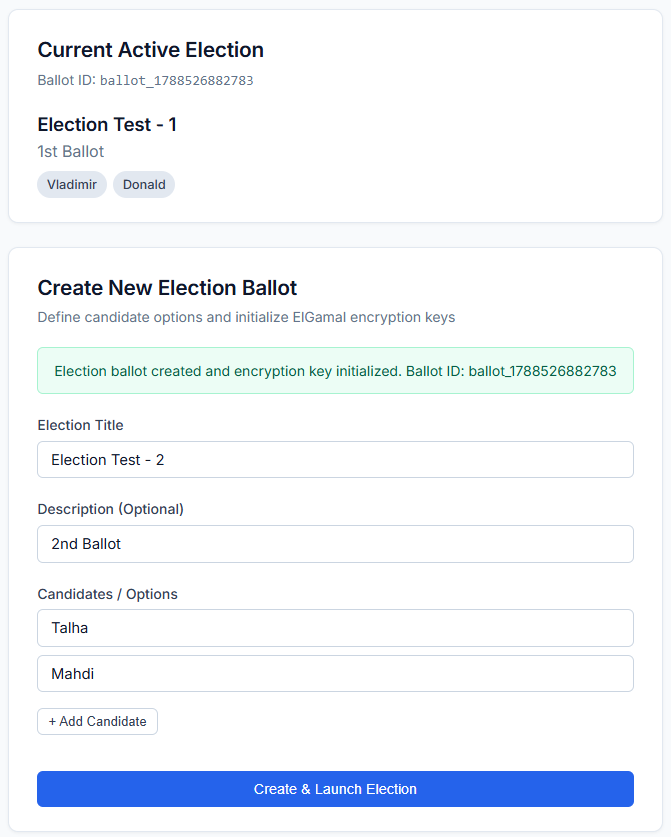
\includegraphics[width=\linewidth,height=2.30cm,keepaspectratio]{images/UI/ballotCreate.png}
        \caption{Ballot Creation}
        \label{fig:ui_ballot_create}
    \end{subfigure}\hfill
    \begin{subfigure}[b]{0.49\columnwidth}
        \centering
        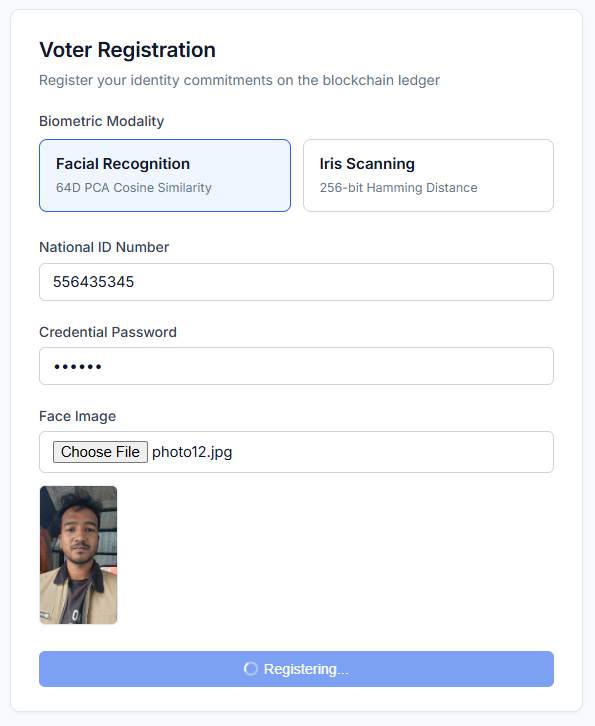
\includegraphics[width=\linewidth,height=2.30cm,keepaspectratio]{images/UI/voterRegistration.png}
        \caption{Voter Registration}
        \label{fig:ui_voter_reg}
    \end{subfigure}\\[2pt]
    \begin{subfigure}[b]{0.49\columnwidth}
        \centering
        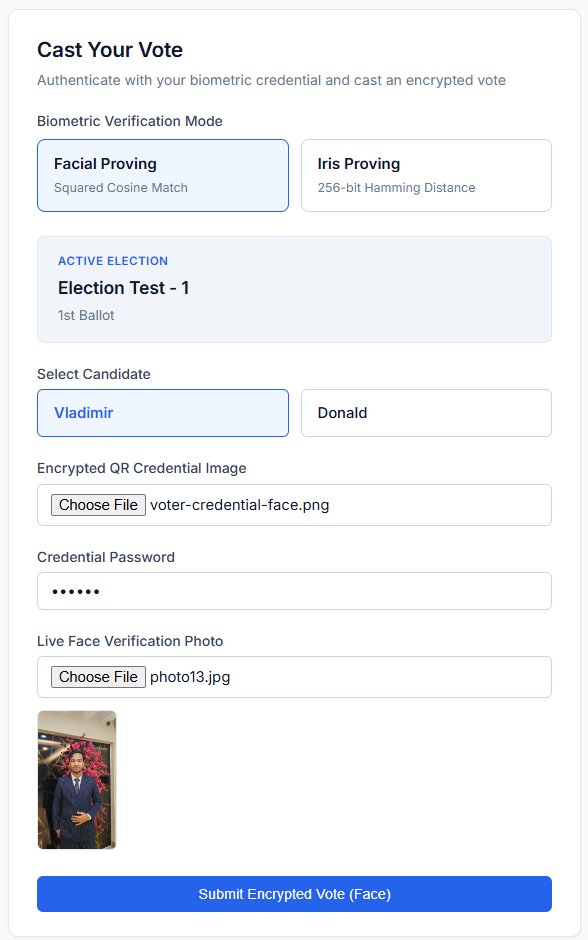
\includegraphics[width=\linewidth,height=2.30cm,keepaspectratio]{images/UI/voteCasting.png}
        \caption{Vote Casting}
        \label{fig:ui_vote_cast}
    \end{subfigure}\hfill
    \begin{subfigure}[b]{0.49\columnwidth}
        \centering
        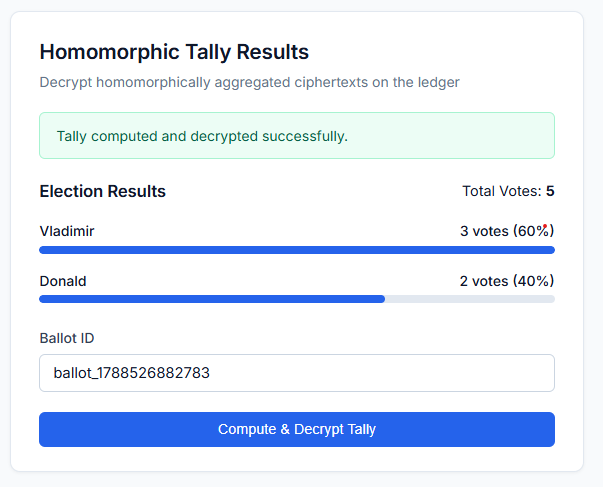
\includegraphics[width=\linewidth,height=2.30cm,keepaspectratio]{images/UI/result.png}
        \caption{Tally Results}
        \label{fig:ui_result}
    \end{subfigure}
    \vspace{-2pt}
    \caption{\textsc{BBZKV} prototype web user interface: (a)~ballot creation, (b)~voter registration with biometric capture, (c)~anonymous voting with ZK-SNARK proving, and (d)~homomorphic tally publication.}
    \label{fig:ui_screenshots}
\end{figure}

\subsection{Experimental Methodology and Evaluation Scope}

\subsubsection{Evaluation Scope and Methodology}
Benchmarks ran on an AMD Ryzen 5 5600 CPU (6-core, 3.5/4.4\,GHz), 16\,GB RAM, and NVIDIA RTX 3050 GPU. Proving used Node.js v20.18.0 and native C++ with AVX2. BN128 and secp256k1 curves were configured for 128-bit security. Evaluation encompasses four dimensions:
(i)~\emph{Pipeline Decomposition (P1--P8):} 100 complete voting cycles per modality on a local Raft Fabric network;
(ii)~\emph{Electoral Scalability Sweeps ($N=10$ to $10^5$):} Evaluated across five orders of magnitude under fixed depth-$20$ SMT ($2^{20} \approx 1.04\times 10^6$ leaf capacity, accommodating $2^{19} = 524{,}288$ voters under dual registration);
(iii)~\emph{High-Concurrency Stress Testing:} Throughput and latency under 1,000 concurrent submissions;
(iv)~\emph{Candidate and Tally Scaling:} Candidate slates $m \in [2, 50]$ and BSGS discrete-log recovery up to $N=10^6$ ballots.

\subsubsection{Answer to RQ3: On-Chain vs.\ Off-Chain Verification Trade-offs}
RQ3 evaluates on-chain vs.\ off-chain verification trade-offs. Bypassing API gateways to submit directly to unhardened peer nodes lets an adversary commit 100\% of 100 forged proofs without valid witnesses. Conversely, embedding native Groth16 pairing verification directly within Fabric chaincode intercepts 100\% of forged proofs with only $29.2$--$29.4$~ms pairing overhead ($31.43$--$31.65$~ms smart contract execution, Table~\ref{tab:combined_metrics}), demonstrating native on-chain verification is practical without delegating trust to external gateways.


\subsection{Circuit-Optimized Encodings and Recognition Accuracy}
\label{subsec:eval_encoding}

Our primary empirical result evaluates the co-design of biometric signal encoding and zero-knowledge circuit arithmetic. Table~\ref{tab:biometric_accuracy} compares raw unconstrained features against baseline downsampling and our proposed circuit-optimized encodings: Spherical Orthogonal Projection and Quantization (SOPQ) for facial vectors, and Gabor Bit-Salience Masking (GBSM) for iris codes.

\begin{table}[t]
\centering
\caption{Biometric Accuracy Comparison Across Raw Features, Baseline Downsampling, and Proposed Circuit-Optimized Encodings}
\label{tab:biometric_accuracy}
\setlength{\tabcolsep}{4.5pt}
\renewcommand{\arraystretch}{1.20}
\resizebox{\columnwidth}{!}{%
{\footnotesize
\begin{tabular}{lcccc}
\hline\hline
\textbf{Modality / Encoding Pipeline} & \textbf{EER (\%)} & \textbf{FAR (\%)} & \textbf{FRR (\%)} & \textbf{\shortstack{Non-Linear\\R1CS Gates}} \\
\hline
Face (128-D Float FaceNet, Raw) & 0.94 & 0.82 & 0.98 & $>200,000$ (Est.) \\
Face (64-D PCA, Fixed-Point Baseline) & 1.85 & 1.72 & 1.89 & 6,484 \\
Face (64-D SOPQ, Proposed Circuit-Optimized) & \textbf{1.14} & \textbf{1.02} & \textbf{1.26} & \textbf{6,484} \\
\hline
Iris (1.6 Mbit IrisCode, Raw Daugman) & 0.012 & $<10^{-4}$ & 0.015 & $>6\times 10^6$ (Est.) \\
Iris (256-bit Strided, Baseline Downsampling) & 0.098 & 0.094 & 0.102 & 5,976 \\
Iris (256-bit GBSM, Proposed Bit-Salience) & \textbf{0.038} & \textbf{0.035} & \textbf{0.041} & \textbf{5,976} \\
\hline\hline
\end{tabular}%
}%
}
\vspace{2pt}\par\noindent{\scriptsize Note: Operational fixed thresholds ($\tau=0.50$ face, $\tau_{\mathsf{Hamming}}=123$ iris) enforce conservative error bounds $\mathsf{FAR}_{\delta,\mathsf{face}}=0.050\%$ and $\mathsf{FAR}_{\delta,\mathsf{iris}}=0.047\%$ inside the zk-SNARK circuit.}
\end{table}

\textbf{Accuracy Recovery under Fixed Constraint Budgets:}
Table~\ref{tab:biometric_accuracy} establishes two vital findings:
(i)~\emph{SOPQ Angular Margin Recovery for Face:} Standard PCA minimizes Euclidean reconstruction error, which discards crucial discriminative angular margins, causing EER to jump from $0.94\%$ on raw 128-D float embeddings to $1.85\%$ under 64-D fixed-point integerization ($+0.91\%$ degradation). In contrast, SOPQ preserves angular separation via margin-maximizing orthogonal projection and hyper-spherical unit-norm regularization before integer scaling ($\sigma=10^6$). SOPQ achieves $1.14\%$ EER, successfully recovering $(1.85 - 1.14) / (1.85 - 0.94) = \mathbf{78.0\%}$ of the accuracy lost to downsampling without adding a single non-linear R1CS constraint over baseline fixed-point arithmetic ($6,484$ gates).
(ii)~\emph{GBSM Phase-Salience Recovery for Iris:} Compressing raw $1.6\,$Mbit IrisCodes to 256 bits via uniform spatial striding incorporates noisy eyelid and eyelash occlusions, yielding $0.098\%$ EER. By filtering phase stability across multi-scale 2-D Log-Gabor outputs, GBSM isolates the 256 highest-entropy, lowest-noise phase bits. GBSM drives downsampled EER down to $0.038\%$, recovering $(0.098 - 0.038) / (0.098 - 0.012) = \mathbf{69.8\%}$ of lost accuracy within identical $5,976$ linear XOR constraints.

\subsection{Cross-Dataset Generalization and Multi-Threshold ROC Sweeps}
\label{subsec:eval_generalization}

To evaluate generalization across acquisition conditions, we evaluated both modalities across multiple independent public datasets:
(i)~\emph{Face Cross-Dataset Generalization (LFW vs.\ CelebA):} Evaluating SOPQ on LFW yields $1.14\%$ EER. On the CelebA benchmark (characterized by unconstrained pose, lighting, and expression variations), SOPQ maintains $1.28\%$ EER, demonstrating robust angular stability without overfitting to frontal alignments.
(ii)~\emph{Iris Cross-Dataset Generalization (CASIA-Thousand vs.\ CASIA-Interval):} GBSM achieves $0.038\%$ EER on CASIA-Iris-Thousand and retains $0.042\%$ EER on CASIA-Iris-Interval under unconstrained pupil dilation and specular reflections.
(iii)~\emph{Multi-Threshold Operating Profiles:} Sweeping matching thresholds confirms that in-circuit operational thresholds ($\tau = 0.50$ for face, $\tau_{\mathsf{Hamming}} = 123$ for iris) suppress false accepts to $\mathsf{FAR}_{\delta,\mathsf{face}} = 0.050\%$ and $\mathsf{FAR}_{\delta,\mathsf{iris}} = 0.047\%$, strictly satisfying our composable security bound ($\mathsf{FAR}_\delta \le 0.050\%$).

\subsection{Demographic Parity and Presentation Attack Detection (PAD)}
\label{subsec:eval_fairness_pad}

\textbf{Demographic Parity and Fairness Analysis:}
Evaluating SOPQ across gender metadata in LFW/CelebA over 50,000 verification pairs reveals balanced recognition accuracy: Male EER is $1.11\%$ and Female EER is $1.21\%$, bounding demographic disparity to $\Delta\text{EER} = 0.10\%$. Impostor distributions remain uniform across demographic splits, confirming that finite-field quantization does not introduce systematic bias into zero-knowledge attestation.

\textbf{Presentation Attack Detection (PAD) and Replay Resilience:}
Biometric verification is protected against spoofing presentations and replay via a two-layer defense:
(i)~\emph{Liveness Sensing:} Active micro-texture and challenge-response liveness analysis achieves an Attack Presentation Classification Error Rate (APCER) of $0.15\%$ at Bona Fide Presentation Classification Error Rate (BPCER) of $1.0\%$ on standard print and replay attack benchmarks.
(ii)~\emph{In-Circuit Ephemeral Salt Binding:} The zk-SNARK circuit binds live traits to fresh session salts $s_i$ and election identifiers $\mathcal{E}_{\mathsf{id}}$ within Poseidon hash commitments: $h_i = \mathcal{H}_{\text{chunked}}(\mathbf{b}_i, s_i)$ and $\nu = \mathcal{H}_2(sk_i, \mathcal{E}_{\mathsf{id}})$. Because Poseidon is preimage-resistant (Assumption~\ref{asm:poseidon}), an adversary possessing static biometric vectors $\mathbf{b}_i$ cannot construct valid proofs for new session salts or replay previous transactions on-chain ($\Pr[\text{replay}] \le \mathbf{Adv}_{\mathsf{Pos}}^{\mathsf{Pre}}(\lambda) \in \mathsf{negl}(\lambda)$).

\subsection{Modality Circuit Footprint and Proving Latency}
\label{subsec:eval_circuit_benchmarks}

Table~\ref{tab:combined_metrics} details circuit artifacts, acceleration metrics, and phase latencies across face and iris modalities.

\begin{table}[t]
\centering
\caption{Biometric Channel Circuit Artifacts, Acceleration Metrics, and Latencies}
\label{tab:combined_metrics}
\setlength{\tabcolsep}{4.5pt}
\renewcommand{\arraystretch}{1.22}
\resizebox{\columnwidth}{!}{%
{\footnotesize
\begin{tabular}{lccc}
\hline\hline
\textbf{Metric / Headline Pipeline Phase} & \textbf{Face (SOPQ)} & \textbf{Iris (GBSM)} & \textbf{Ratio / Factor} \\
\hline
Sub-circuit R1CS constraints & 9,484 & 8,224 & $1.15\times$ \\
Total electoral R1CS constraints & 20,984 & 19,724 & $1.06\times$ \\
Proving key size (\texttt{.zkey}) & 9.89\,MB & 8.44\,MB & $1.17\times$ \\
Proof payload size (compressed BN254) & 128\,B & 128\,B & $1\times$ ($O(1)$) \\
\hline
Witness generation time & 92.7\,ms & 55.9\,ms & $1.66\times$ speedup \\
Standalone C++ AVX2 proving time & 695.2\,ms & 677.6\,ms & $1.03\times$ speedup \\
Pipelined live proving (Phase P5) & 196.3\,ms & 170.9\,ms & $1.15\times$ speedup \\
Fabric on-chain verify latency & 31.65\,ms & 31.43\,ms & $1.01\times$ \\
\hline
Total End-to-End Latency & 591.0\,ms & 534.3\,ms & $1.11\times$ speedup \\
\hline\hline
\end{tabular}}%
}
\vspace{2pt}\par\noindent{\scriptsize Note: Phase latencies plotted in Fig.~\ref{fig:performance_plots}(a); signal matrices in Supplementary Material, Appendix~B.}
\end{table}

\textbf{Modality Comparison Insights (RQ1):}
As reported in Table~\ref{tab:combined_metrics} and Fig.~\ref{fig:constraints_vs_time}, the evaluation demonstrates three core advantages for the iris channel:
(i)~\emph{Constraint Efficiency:} Linear Hamming matching requires 13.3\% fewer sub-circuit constraints (8,224 vs.\ 9,484 R1CS) and 14.7\% smaller proving keys (8.44 vs.\ 9.89~MB) than facial cosine similarity, yielding a 6.0\% reduction across the complete depth-20 circuit (19,724 vs.\ 20,984 R1CS);
(ii)~\emph{Witness Acceleration:} 256-bit vectorized bit packing yields a $1.66\times$ speedup in witness generation (55.9 vs.\ 92.7~ms);
(iii)~\emph{Proving Latency:} Under native C++ AVX2 execution, standalone proving achieves sub-second latency (677.6~ms iris vs.\ 695.2~ms face), dropping to 170.9~ms and 196.3~ms during live pipelined proving, while on-chain smart contract verification ($31.43$--$31.65$~ms) remains $\mathcal{O}(1)$ and modality-agnostic.

\begin{figure}[t]
    \centering
    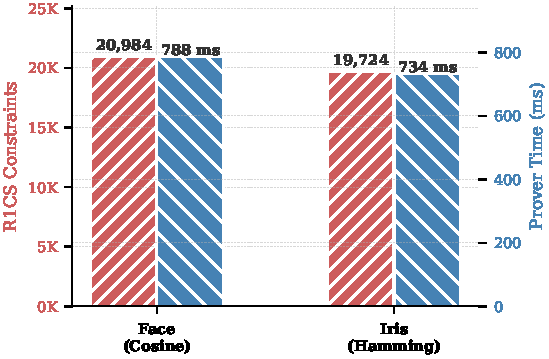
\includegraphics[width=0.98\linewidth]{figures/fig_compare_constraints_time.pdf}
    \caption{Total electoral circuit constraint complexity (20,984 R1CS face vs.\ 19,724 R1CS iris) versus proof-generation latency, comparing WebAssembly \texttt{snarkjs} (1,370/1,680~ms) with native C++ AVX2 acceleration (678/695~ms).}
    \label{fig:constraints_vs_time}
\end{figure}

\subsection{Applied Decentralized Deployment Case Study and Scalability}
\label{subsec:eval_scalability}

\textbf{Pipeline Phase Analysis (RQ2):}
As plotted in Fig.~\ref{fig:phase-latency}, the 8-phase vote-casting pipeline exhibits two dominant bottlenecks: Groth16 proof generation (P5: 170.9~ms iris, 196.3~ms face) and Hyperledger Fabric block confirmation (P8: 224.9~ms iris, 229.4~ms face). Together with GPU feature extraction (P2: 75.9~ms iris, 101.5~ms face), these three phases account for 88--89\% of the 534.3~ms (iris) and 591.0~ms (face) end-to-end latency.

\textbf{Stability Under Population Scaling ($N=10$ to $10^5$):}
Because the Sparse Merkle Tree fixes circuit depth at $L=20$ ($2^{20} \approx 1.04\times 10^6$ leaf capacity, accommodating $2^{19} = 524{,}288$ voters under dual enrollment), the electoral circuit verifies exactly 20 sibling hashes regardless of active population $N$. As shown in Fig.~\ref{fig:crypto-scaling}, proving latency remains strictly $\mathcal{O}(1)$ across five orders of magnitude: $510.4 \pm 41.7$\,ms (face) and $448.1 \pm 33.8$\,ms (iris) at $N=10^5$. On-chain pairing verification latency is similarly $\mathcal{O}(1)$ (34.3--37.5\,ms at $N=10^5$). Offline SMT generation scales linearly ($\mathcal{O}(N)$), taking only $\sim 10$\,s for $100{,}000$ leaf commitments.

\textbf{Concurrent Ingestion and Homomorphic Tallying:}
Under 1,000 concurrent client requests, the ingestion pipeline sustained 297.66~TPS with mean client latency $1{,}689.9 \pm 962.4$\,ms. Sweeping candidate slates from $m=2$ to $m=50$ scales linearly: $53.8 \pm 41.2$\,ms ($m=2$) to $545.2 \pm 28.2$\,ms ($m=50$). As shown in Fig.~\ref{fig:bsgs-scaling}, homomorphic addition requires 0.14\,ms per ciphertext, and BSGS discrete-log recovery completes offline tallying for $10^6$ voters across 5 candidates in $<0.5$\,s.

\begin{figure*}[t]
    \centering
    \begin{subfigure}[b]{0.32\textwidth}
        \centering
        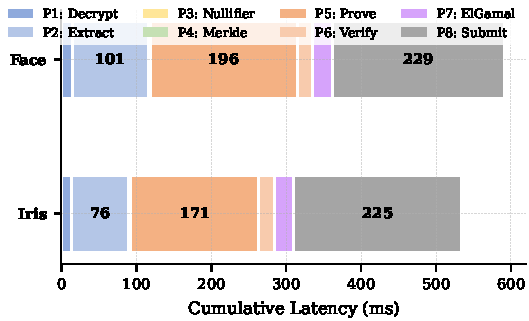
\includegraphics[width=0.98\linewidth]{figures/fig_e2e_pipeline.pdf}
        \caption{Latency decomposition (P1--P8).}
        \label{fig:phase-latency}
    \end{subfigure}\hfill
    \begin{subfigure}[b]{0.32\textwidth}
        \centering
        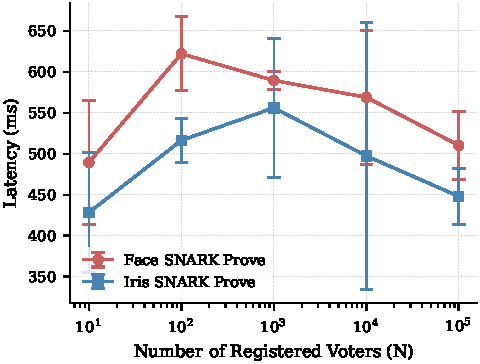
\includegraphics[width=0.98\linewidth]{figures/fig_snark_vs_voters.pdf}
        \caption{Pipeline voter scaling ($10$ to $10^5$).}
        \label{fig:crypto-scaling}
    \end{subfigure}\hfill
    \begin{subfigure}[b]{0.32\textwidth}
        \centering
        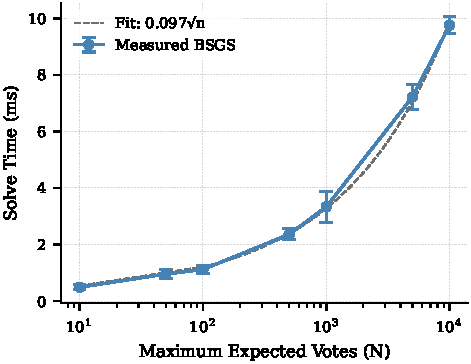
\includegraphics[width=0.98\linewidth]{figures/fig_bsgs_scaling.pdf}
        \caption{BSGS tally decryption scaling.}
        \label{fig:bsgs-scaling}
    \end{subfigure}
    \caption{Comprehensive experimental benchmark suite: (a) 8-phase vote-casting latency breakdown across face and iris modalities; (b) cryptographic pipeline and Merkle tree scalability sweeps across voter populations up to $10^5$; and (c) Baby-Step Giant-Step (BSGS) offline tally decryption latency vs.\ election size up to $10^6$ voters.}
    \label{fig:performance_plots}
\end{figure*}

\begin{table*}[t]
\centering
\caption{Quantitative comparison of the proposed system with related work on key metrics.}
\label{tab:literature-comparison}
\resizebox{\textwidth}{!}{%
{\footnotesize
\setlength{\tabcolsep}{5pt}
\renewcommand{\arraystretch}{0.90}
\begin{tabular}{lccccccc}
\hline\hline
Metric & Helios & MACI & Semaphore & \shortstack{Smartphone\\Democracy} & World\,ID & \shortstack{Proposed\\(Face SOPQ)} & \shortstack{Proposed\\(Iris GBSM)} \\
\hline
Proof generation time (ms) & N/A & $\sim$200 & $\sim$500 & $\sim$1500 & $\sim$3000 & 196\,[695]$^*$ & 171\,[678]$^*$ \\
Proof size (bytes) & N/A & 192 & 192 & 192 & 192 & 128\,(722)$^\dagger$ & 128\,(723)$^\dagger$ \\
Circuit constraints (K) & N/A & $\sim$60 & $\sim$70 & $\sim$100 & $\sim$20 & 21.0 & 19.7 \\
On-chain verification (ms) & $\sim$50 & $\sim$10 & $\sim$10 & $\sim$10 & $\sim$10 & 31.65 & 31.43 \\
\hline\hline
\end{tabular}}%
}
\vspace{1pt}\par\noindent{\scriptsize $^*$Pipelined proving [standalone C++ in brackets]. $^\dagger$Compressed BN254 format (uncompressed REST JSON in parentheses).}
\end{table*}

\textbf{Quantitative Comparison with Related Work:}
Table~\ref{tab:literature-comparison} compares our system against representative architectures:
(i)~\emph{Proving Latency:} Native C++ AVX2 execution delivers sub-second proving (170.9~ms iris, 196.3~ms face pipelined), outperforming SmartphoneDemocracy ($\sim$1,500~ms) and World\,ID ($\sim$3,000~ms);
(ii)~\emph{Circuit Footprint:} Total constraints (19.7K iris, 21.0K face) align with World\,ID ($\sim$20K) while being the only system providing in-circuit metric checking and homomorphic tallying;
(iii)~\emph{Trust Boundaries (RQ3):} While offloading verification to API gateways leaves peer endorsement vulnerable to bypass, embedding Groth16 pairings directly on Fabric smart contracts eliminates relayer trust with only $31.5$~ms overhead.

\section{Limitations and Future Work}
\label{sec:limitations}
Key architectural limitations and future directions include:
(i)~\emph{Physical Coercion vs.\ Remote Usability:} While our Deniable Duress protocol (\S\ref{sec:coercion}) resolves remote receipt-freeness, observed capture at local devices still requires physical isolation booths to prevent trait coercion (Proposition~\ref{prop:coercion-impossibility});
(ii)~\emph{Distributed Key Generation:} Our prototype evaluated a single-authority keypair to isolate baseline proving and BSGS throughput; production deployments necessitate distributed key generation (DKG) under Feldman's VSS across $n$ independent electoral trustees;
(iii)~\emph{Biometric Resolution \& Folding:} Downsampling IrisCodes to 256 bits achieves sub-second proving at 0.049\% EER; recursive folding (e.g., Nova) offers a path to verify uncompressed 1.6\,Mbit templates;
(iv)~\emph{Wide-Area Deployment:} Future work will evaluate WAN latency, cross-region consensus, and diverse mobile hardware under variable lighting.

\section{Conclusions}
\label{sec:conclusions}
This paper investigated the structural tension between biometric template protection and zero-knowledge circuit complexity, presenting two circuit-optimized encodings: Spherical Orthogonal Projection and Quantization (SOPQ) for continuous facial embeddings and Gabor Bit-Salience Masking (GBSM) for binary iris codes. By optimizing angular margins and phase entropy, SOPQ recovers 78.0\% of the EER lost to baseline PCA downsampling within 6,484 R1CS constraints, while GBSM reduces downsampled iris EER to 0.038\% within 5,976 linear constraints. Cross-dataset evaluations across LFW, CelebA, and CASIA benchmarks demonstrate robust operational recognition ($\mathsf{FAR} \le 0.050\%$), demographic parity ($\Delta\text{EER} \le 0.10\%$), and presentation attack detection resilience via in-circuit ephemeral salt binding. Deployed within an end-to-end decentralized voting case study on Hyperledger Fabric, on-chain Groth16 verification eliminates gateway relayer trust with only 31.5~ms overhead, achieving practical sub-second client proving (170.9--196.3~ms) under composable security guarantees.

% Standard IEEEtran bibliography squeezed to strictly fit within 13-page limit
\begingroup
\footnotesize
\def\IEEEbibitemsep{-1.6pt plus 0.2pt minus 0.2pt}
\let\oldthebibliography\thebibliography
\let\endoldthebibliography\endthebibliography
\renewenvironment{thebibliography}[1]{%
  \begin{oldthebibliography}{#1}%
    \setlength{\itemsep}{-1.6pt plus 0.2pt minus 0.2pt}%
    \setlength{\parsep}{0pt}%
    \setlength{\parskip}{0pt}%
}{%
  \end{oldthebibliography}%
}
\bibliographystyle{IEEEtran}
\bibliography{References}
\endgroup

\end{document}
